\chapter{Случайные события}

\section{Определение пространства элементарных исходов, примеры. Понятие события (нестрогое), следствие события, невозможное и достоверное событие, примеры. Операции над событиями. Сформулировать классическое определение вероятности и доказать его следствия}

\subsection{Определение пространства элементарных исходов, примеры}
Пространство элементарных исходов - это множество всех элементарных исходов $\Omega$.\\

Элементарный исход - каждый неделимый результат случайного эксперимента.\\

Примеры:\\
1) Бросают монету. Возожные исходы включают в себя орла (О) и решку (Р), тогда пространство элементарных исходов будет $\Omega = \{$О$, $Р$\}$. $|\Omega| = 2$ - мощность множества $\Omega$.

2) Из колоды в 36 карт последовательно извлекают две карты.
Возможные исходы: $\Omega = \{(x_1, x_2): x_1, x_2 \in \{1, .. , 36\}, x_1 \neq x_2$\}, $x_i$ - номер карты, которая появилась при i-ом извлечении. $|\Omega| = 36 \cdot 35$.

\subsection{Понятие события (нестрогое), следствие события, невозможное и достоверное событие, примеры}

Нестрогое понятие события: событие - любое подмножество множества всех элементарных исходов $\Omega$.\\

Следствие события - Событие B называется следствием события A, если из того, что произошло событие А следует, что произошло событие B. Другими словами B называется следствием A, если A$\subseteq$B.\\

\begin{figure}[H]
	\center{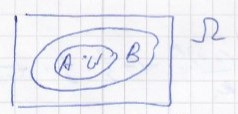
\includegraphics[scale=2.0]{AinB}}
	\caption{Отношения множеств A и B}
\end{figure}

Невозможные и достоверные события - любое множество $\Omega$ содержит два подмножества - $\varnothing, \Omega$. Соответствующие события называются невозможными ($\varnothing$) и достоверными ($\Omega$).\\

Невозможное событие - невозможным событием, связанным с опытом S, называется такое событие, которые обязательно не произойдёт в результате опыта S.\\

Достоверное событие - достоверным событием, связанным с опытом S, называется такое событие, которое обязательно произойдёт в результате опыта S.\\

Несовместимые события - события называются несовместимыми, если в результате опыта они не могут наступить одновременно.\\

Пример несовместимых событий:
Из урны, содержащих 2 красных и 3 синих шара, вынимают случайным образом один шар.

А = \{извлечён белый шар\} = $\varnothing$

B = \{извлечён красный или синий шар\} = $\Omega$

\subsection{Операции над событиями}
События являются множествами, следовательно к ним применимы операции над множествами: $\cap, \cup, \neg, \backslash, \triangle$.

В теории вероятностей используется следующая терминология:\\
$A \cup B$ - $A + B$ - сумма событий (объединение, выполняется хотя бы одно из событий)\\
$A \cap B$ - $A \cdot B$ - произведение событий (пересечение, выполняются оба события)\\
$A \backslash B$ - разность событий событий\\
$\neg A = \Omega \backslash A$ - дополнение события А \\

Операции над событиями:
\begin{enumerate}
\item A + B = B + A - коммутативность
\item $A \cdot B = B \cdot A$ - коммутативность
\item (A + B) + C = A + (B + C) - ассоциативность
\item $(A \cdot B) \cdot C = A \cdot (B \cdot C)$ - ассоциативность
\item $A \cdot A = A$ - идемпотентность
\item $A \cdot \neg A = \varnothing$
\item $A \cdot \varnothing = \varnothing$
\item $A \cdot \Omega = A$
\item $ A + A = A$ - идемпотентность
\item $A + \neg A = \Omega$
\item $A + \varnothing = A$
\item $A + \Omega = \Omega$
\item $A \backslash B = A \cdot \neg B$
\item $\neg \Omega = \varnothing$
\item $\neg \varnothing = \Omega$
\item $A \cdot (B + C) = A \cdot B + A \cdot C$ - дистрибутивность
\item $\neg(\neg(A)) = A$
\item $\neg(A + B) = \neg A \cdot \neg B$ - де Морган
\item $\neg(A \cdot B) = \neg A + \neg B$ - де Морган
\end{enumerate}

\subsection{Сформулировать классическое определение вероятности и доказать его следствия}

Классическое определение вероятности:\\
1) Пусть $|\Omega| = N < \infty$\\
2) По условиям эксперимента нет объективных оснований предпочесть какой-нибудь элементарный исход остальным - говорят, что все элементарные исходы равновероятны.\\
Тогда вероятностью события $A \subseteq \Omega$ называется число $P(A) = \frac{N_{A}}{N}$, где $N_{A} = |A|$\\

Свойства вероятности из классического определения:\\
1) $P(A) \geqslant 0$\\
Доказательство:\\
$P(A) = \frac{N_{A}}{N}, N_{A} \geqslant 0, N > 0 \Rightarrow P(A) \geqslant 0$\\
2) $P(\Omega) = 1$\\
Доказательство:\\
$P(\Omega) = \frac{|\Omega|}{N} = \frac{N}{N} = 1$\\
3) Если AB = $\varnothing$, то P(A + B) = P(A) + P(B)\\
Доказательство:\\
По формуле включений и исключений: |A + B| = |A| + |B| - |AB| = |A| + |B|, так как по условию |AB| = 0. Таким образом $N_{A + B} = N_{A} + N_{B}$ и $P(A + B) = \frac{N_{A + B}}{N} = \frac{N_{A} + N_{B}}{N} = P(A) + P(B)$

\section{Опреление пространства элементарных исходов, примеры. Понятиие события (нестрогое). Сформулировать геометрическое и статистическое определения вероятности. Достоинства и недостатки этих определений}

\subsection{Определение пространства элементарных исходов, примеры}
Рассмотрено в пункте 1.1.1

\subsection{Понятие события (нестрогое)}
Рассмотрено в пункте 1.1.2

\subsection{Сформулировать геометрическое и статистическое определения вероятности. Достоинства и недостатки этих определений}

Геометрическое определение вероятности - геометрическое определение обобщает классическое определение на случай, когда $\Omega$ является бесконечным множеством в $R^{n}$ - n-мерном пространстве, имеющем ненулевой объём.

Пусть $A \subseteq R^{n}$. Через $\mu(A)$ будем обозначать меру множества А:\\
n = 1, $\mu(A)$ - длина,\\
n = 2, $\mu(A)$ - площадь,\\
n = 3, $\mu(A)$ - объём,\\
...\\

Пусть:\\
1) $\Omega \subseteq R^{n}, \mu(\Omega) < \infty$\\
2) $A \subseteq \Omega$\\

Тогда по геометрическому определению вероятности - вероятностью события А называется число $P(A) = \frac{\mu(A)}{\mu(\Omega)}$.\\

Достоинством геометрического определения вероятности является то, что для него остаются в силе свойства 1-3 классчического определения вероятности.\\
Недостатком геометрического определения вероятности является то, что оно не применимо в случае, когда отдельные области являются более предпочтительными.\\

Статистическое определение вероятности:\\
Пусть:\\
1) случайный эксперимент повторён n раз.\\
2) при этом событие А произошло $n_{A}$ раз.\\

Тогда по статистическому определению вероятности - вероятностью события А называется эмпирический (то есть полученный опытным путём) предел отношения $\frac{n_{A}}{n}$ при $ n \rightarrow \infty$.\\

Недостатком статистического определения является то, что опыт не может быть повторён бесконечное число раз. Такое определение не даёт достаточной основы для дальнейшего развития математической теории.\\

\section{Определение пространства элементарных исходов, примеры. Сформулировать определение сигма-алгебры событий. Доказать простейшие свойства сигма-алгебры. Сформулировать аксиоматическое определение вероятности.}

\subsection{Определение пространства элементарных исходов, примеры}
Рассмотрено в пункте 1.1.1

\subsection{Сформулировать определение сигма-алгебры событий}
Определение сигма-алгебры событий:\\
Пусть:\\
1) $\Omega$ - пространство элементарных исходов.\\
2) $\mathcal{B}$ - некоторый набор подмножеств множества $\Omega$, $\mathcal{B} \neq \varnothing$\\

Тогда $\mathcal{B}$ называется сигма-алгеброй, если:\\
1) $A \in \mathcal{B} \Rightarrow \overline{A} \in \mathcal{B}$\\
2) $A_{1}, A_{2} ... A_{n} \in \mathcal{B} \Rightarrow A_{1} + A_{2} + ... + A_{n} \in \mathcal{B}$\\ 

Простейшие свойства сигма-алгебры событий из определения:\\
1) $\Omega \in \mathcal{B}$\\
Доказательство:\\
Так как $\mathcal{B} \neq \varnothing$, то есть некоторое производное множество $A \in \mathcal{B}$, в силу первого определения $\overline{A} \in \mathcal{B}$, в силу второго $\Omega = A + \overline{A} \in \mathcal{B}$\\
2) $\varnothing \in \mathcal{B}$\\
Доказательство:\\
Так как $\Omega \in \mathcal{B} \Rightarrow \overline{\Omega} \in \mathcal{B} \Rightarrow \varnothing \in \mathcal{B}$\\
3) если $A_{1}, A_{2} ... A_{n} \in \mathcal{B} \Rightarrow A_{1} \cdot A_{2} \cdot ... \cdot A_{n} \in \mathcal{B}$\\
Доказательство:\\
$A_{1}, A_{2} ... A_{n} \in \mathcal{B} \Rightarrow $ (по первому пункту определения сигма-алгебры) $ \overline{A_{1}}, \overline{A_{2}} ... \overline{A_{n}} \in \mathcal{B} \Rightarrow $ (по второму пункту определения сигма-алгебры) $ \overline{A_{1}} + \overline{A_{2}} + ... + \overline{A_{n}} \in \mathcal{B} \Rightarrow $ (по первому пункту определения сигма-алгебры) $ \overline{\overline{A_{1}} + \overline{A_{2}} + ... + \overline{A_{n}}} \in \mathcal{B} \Rightarrow $ (по закону де Моргана) $ A_{1} \cdot A_{2} \cdot ... \cdot A_{n} \in \mathcal{B} $\\
4) если $A, B \in \mathcal{B}$, то $A \backslash B \in \mathcal{B}$\\
Доказательство:\\
По свойствам операций над событиями - $ A \backslash B = A \cdot \overline{B}$. Так как $ A \in \mathcal{B}, B \in \mathcal{B}, \overline{B} \in \mathcal{B}$ по третьему свойству сигма-алгебры событий - $ A \cdot \overline{B} \in \mathcal{B}$

\subsection{Сформулировать аксиоматическое определение вероятности}

Аксиоматическое определение вероятности:\\
Пусть:\\
1) $\Omega$ - пространство элементарных исходов\\
2) $\mathcal{B}$ - некоторая $\sigma$-алгебра событий\\

Тогда по аксиоматическому определению вероятности - вероятностью (вероятностной мерой) называют функцию $P : \mathcal{B} \rightarrow \mathcal{R}$, которая обладает следующими свойствами:\\
1) Аксиома неотрицательности:\\
$\forall A \in \mathcal{B}$ $P(A) \geqslant 0$\\
2) Аксиома нормированности:\\
$P(\Omega) = 1$\\
3) Расширенная аксиома сложения:\\
Для любой последовательности событий $A_{1}, ..., A_{n} \in \mathcal{B}$, которые попарно несовместны, справедливо:\\
$P(A_{1} + A_{2} + ... + A_{n}) = P(A_{1}) + P(A_{2}) + ... + P(A_{n})$

\section{Определение пространства элементарных исходов, примеры. Сформулировать определение сигма-алгебры событий. Сформулировать аксиоматическое определение вероятности и доказать простейшие свойства вероятности}

\subsection{Определение пространства элементарных исходов, примеры}
Рассмотрено в пункте 1.1.1

\subsection{Сформулировать определение сигма-алгебры событий}
Рассмотрено в пункте 1.3.2

\subsection{Сформулировать аксиоматическое определение вероятности и доказать простейшие свойства вероятности}
Аксиоматическое определение вероятности:\\
Пусть:\\
1) $\Omega$ - пространство элементарных исходов\\
2) $\mathcal{B}$ - некоторая $\sigma$-алгебра событий\\

Вероятностью (вероятностной мерой) называют функцию $P : \mathcal{B} \rightarrow \mathcal{R}$, которая обладает следующими свойствами:\\
1) Аксиома неотрицательности:\\
$\forall A \in \mathcal{B}$  $P(A) \geqslant 0$\\
2) Аксиома нормированности:\\
$P(\Omega) = 1$\\
3) Расширенная аксиома сложения:\\
Для любой последовательности событий $A_{1}, ..., A_{n} \in \mathcal{B}$, которые попарно несовместны, справедливо:\\
$P(A_{1} + A_{2} + ... + A_{n}) = P(A_{1}) + P(A_{2}) + ... + P(A_{n})$\\

Свойства аксиоматического определения вероятности:\\
1) $P(\overline{A}) = 1 - P(A)$\\
$\Omega = A + \overline{A}, A \cdot \overline{A} = \varnothing\\
P(\Omega) = 1 $  (аксиома пункт 2)\\
$P(\Omega) = P(A + \overline{A}) = $ (аксиома пункт 3) $ = P(A) + P(\overline{A})$\\
$P(A) + P(\overline{A}) = 1 \Rightarrow P(\overline{A}) = 1 - P(A)$\\
2) $P(\varnothing) = 0$\\
Доказательство:\\
$\varnothing = \overline{\Omega}$\\
По свойству вероятности 1 (предыдущее свойство) $P(\varnothing) = 1 - P(\Omega) = $ (Аксиома пункт 2) $ 1 - 1 = 0 $\\
3) если $A \subseteq B$, то $P(A) \leqslant P(B)$\\
Доказательство:\\
\begin{figure}[H]
	\center{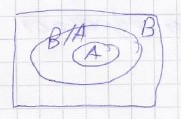
\includegraphics[scale=2.0]{AinB_2}}
	\caption{Отношения множеств A и B}
\end{figure}
$ B = A + (B \backslash A), $ так как $ A \cdot (B \backslash A) = \varnothing, $ то по аксиоме 3: $ P(B) = P(A + B \backslash A) = P(A) + P(B \backslash A) \geqslant P(A) $\\
4) $\forall A \in \mathcal{B}$: $0 \leqslant P(A) \leqslant 1$\\
Доказательство:\\
$P(A) \geqslant 0$ по аксиоме 1 (аксиома неотрицательности).\\
Докажем, что $P(A) \leqslant 1$\\
$A \subseteq \Omega \Rightarrow $ по свойству 3 $ \Rightarrow P(A) \leqslant P(\Omega) = 1$\\
5) $P(A + B) = P(A) + P(B) - P(AB)$\\
Доказательство:\\
a) $A + B = A + (B \backslash A)$, так как $ A \cdot (B \backslash A) = \varnothing $ тогда по аксиоме 3: $ P(A + B) = P(A) + P(B \backslash A)$\\
b) $ B = (B \backslash A) + AB$ так как $(B \backslash A)(AB) = \varnothing$, то $P(B) = P(B \backslash A) + P(AB) \Rightarrow P(B \backslash A) = P(B) - P(AB)$\\
c) $P(A + B) = P(A) + P(B) - P(AB)$\\
6) Теорема сложения n событий:\\
Если $ A_{1}, ... , A_{n}  \in \mathcal{B} $, то $P(A_{1} + ... + A_{n}) = \sum\limits_{i=1}^{n} P(A_{i}) - \sum\limits_{1 \leqslant i < j \leqslant n} P(A_{i} \cdot A_{j}) + \sum\limits_{1 \leqslant i < j < k \leqslant n} P(A_{i} \cdot A_{j} \cdot A_{k}) + ... + (-1)^{n + 1} P(A_{1} \cdot ... \cdot A_{n})$\\
Для n = 3:\\
$P(A + B + C) = P(A) + P(B) + P(C) - P(A \cdot B) - P(B \cdot C) - P(A \cdot C) + P(A \cdot B \cdot C)$\\
Доказательство:\\
Является следствием доказательства 5 и доказывается аналогично формуле включений и исключений.

\section{Сформулировать определение условной вероятности. Доказать, что при фиксированном событии B условная вероятность P(A|B) обладает всеми свойствами безусловной вероятности}

\subsection{Сформулировать определение условной вероятности}
Определение условной вероятности - пусть P(B) > 0. Условной вероятностью осуществления события A, при условии, что произошло B, называют число  $P(A|B) = \frac{P(AB)}{P(B)}$\\ 

\subsection{Доказать, что при фиксированном событии B условная вероятность P(A|B) обладает всеми свойствами безусловной вероятности}
Теорема - при фиксированном событии B условная вероятность удовлетворяет всем аксиомам безусловной вероятности:\\

Зафиксируем событие B, P(B) > 0, и будем рассматривать условную вероятность P(A|B), как функцию события А.\\

1) $P(A|B) \geqslant 0$\\
Доказательство:\\
$P(A|B) = \frac{P(AB)}{P(B)}, P(AB) \geqslant 0$, так как вероятность произведения событий может быть равна нулю, если события несовместны, P(B) > 0, так как B является фиксированным событием, т.е. происходит при любом эксперименте\\
2) $P(\Omega|B) = 1$\\
Доказательство:\\
$P(\Omega|B) = \frac{P(\Omega B)}{P(B)} = \frac{P(B)}{P(B)} = 1$\\
3) Для любого случайного набора попарно независимых событий $A_{1}, ... A_{n}$ имеет место $P(A_{1} + ... + A_{n} | B) = P(A_{1} | B) + ... + P(A_{n} | B)$\\
Доказательство:\\
$P(A_{1} + ... + A_{n} | B) = \frac{P((A_{1} + ... + A_{n}) \cdot B)}{P(B)} = \frac{P(A_{1}B + ... + A_{n}B)}{P(B)} $ (такое преобразование возможно, поскольку B - фиксированное событие, и для условной вероятности это значит, что для каждого события A также выполняется событие B, то есть произведение вероятностей) = по третьей аксиоме = $ \frac{1}{P(B)} [P(A_{1}B) + ... + P(A_{n}B)] $ = $\sum\limits^{n}_{i=1} \frac{P(A_{i}B)}{P(B)} =  \sum\limits^{n}_{i=1} P(A_{i}|B)$\\

Следствия теоремы о том, что при фиксированном событии B условная вероятность P(A|B) обладает всеми свойствами безусловной вероятности:\\
Условная вероятность обладает всеми свойствамии безусловной вероятности:\\
1) $P(\overline{A}|B) = 1 - P(A|B)$\\
2) $P(\varnothing|B) = 0$\\
3) если $A_{1} \subseteq A_{2}$, то $P(A_{1}|B) \leqslant P(A_{2}|B)$\\
4) $0 \leqslant P(A|B) < 1$\\
5) $P(A_{1} + A_{2}|B) = P(A_{1}|B) + P(A_{2}|B) - P(A_{1} A_{2} | B)$\\
6) $P(A_{1} + ... + A_{n}|B) =  \sum\limits_{i=1}^{n} P(A_{i}|B) - \sum\limits_{1 \leqslant i < j \leqslant n} P(A_{i} \cdot A_{j}|B) + \sum\limits_{1 \leqslant i < j < k \leqslant n} P(A_{i} \cdot A_{j} \cdot A_{k}|B) + ... + (-1)^{n + 1} P(A_{i} \cdot ... \cdot A_{n}|B)$\\

Доказательство:\\
Свойства 1-6 для безусловной вероятности следствиями аксиом 1-3, так как условная вероятность удовлетворяет этим аксиомам то для неё будут верны все следствия.

\section{Сформулировать определение условной вероятности. Доказать теорему (формулу) умножения вероятностей. Привести пример использования этой формулы}

\subsection{Сформулировать определение условной вероятности}
Рассмотрено в пункте 1.5.1

\subsection{Доказать теорему (формулу) умножения вероятностей. Привести пример использования этой формулы}
Теорема (формула) умножения вероятностей:\\
Пусть события $A_{1} ... A_{n}$ таковы, что $P(A_{1} ... A_{n - 1}) > 0$. Тогда $P(A_{1} \cdot ... \cdot A_{n}) = P(A_{1}) \cdot P(A_{2} | A_{1}) \cdot P(A_{3} | A_{1} A_{2}) \cdot ... \cdot P(A_{n}|A_{1} ... A_{n-1})$ - формула умножения вероятностей (*).\\

Доказательство:\\
1) Для любого $k \in \{1, ..., n - 1\}$  $ A_{1} \cdot ... \cdot A_{k} \geqslant A_{1} \cdot ... \cdot A_{n-1} \Rightarrow P(A_{1} \cdot ... \cdot A_{k}) \geqslant P(A_{1} \cdot ... \cdot A_{n-1}) > 0 \Rightarrow $ все условные вероятности в формуле умножения вероятностей (*) определены\\
2) $P(A_{1} \cdot ... \cdot A_{n-1} \cdot A_{n}) = P(A_{1} \cdot ... \cdot A_{n-2} \cdot A_{n-1})P(A_{n} | A_{1} \cdot ... \cdot A_{n-1}) = P(A_{1} \cdot ... \cdot A_{n-2})P(A_{n-1} | A_{1} \cdot ... \cdot A_{n-2})P(A_{n}|A_{1} ... A_{n-1}) = ... = P(A_{1})P(A_{2} | A_{1}) \cdot ... \cdot P(A_{n} | A_{1} \cdot ... \cdot A_{n-1})$\\

Пример использования формулы умножения вероятностей:\\
На 7 карточках написаны буквы слова "ШОКОЛАД". Карточки перемешивают и последовательно вынимают три штуки. A = \{карты в порядке появления образуют слово "КОД"\}\\
P(A) = ?\\
Решение:
$A_{1}$ = \{на первой карточке написано "К"\}\\
$A_{2}$ = \{на второй карточке написано "О"\}\\
$A_{3}$ = \{на третьей карточке написано "Д"\}\\
Тогда A = $A_{1} A_{2} A_{3}$. По формуле умножения вероятности:\\
$P(A) = P(A_{1} A_{2} A_{3}) = P(A_{1}) P(A_{2} | A_{1}) P(A_{3} | A_{1} A_{2}) = \frac{1}{7} \frac{2}{6} \frac{1}{5} = \frac{1}{105}$\\
$P(A_{2} | A_{1})$ - 6 карт, карточки с К нет в колоде.\\
$P(A_{3} | A_{1} A_{2})$ - 5 карт, карточек с К и О нет в колоде\\

\section{Сформулировать определение пары независимых событий. Доказать критерий независимости двух событий. Сформулировать определение попарно независимых событий и событий, независисмых в совокупности. Обосновать связть этих свойств}
\subsection{Сформулировать определение пары независимых событий}
Определение пары независимых событий - события A и B называюся независимыми, если P(AB) = P(A) P(B)\\
\subsection{Доказать критерий независимости двух событий}
Критерий независимости двух событий:\\
1) Если P(B) > 0, то A, B - независимы $\Leftrightarrow P(A|B) = P(A)$ (событие B является зафикированным, т.е. происходит всегда. Вследствие чего наступление события A не зависит от наступления события B)\\
2) Если P(A) > 0, то A, B - независимы $\Leftrightarrow P(B|A) = P(B)$\\

Доказательство:\\
В левую сторону - пусть P(AB) = P(A) P(B), тогда $P(A|B) = \frac{P(AB)}{P(B)} = \frac{P(A)P(B)}{P(B)} = P(A)$\\
В правую сторону - пусть P(A|B) = P(A), тогда $P(A|B) = P(A) = \frac{P(AB)}{P(B)} \Rightarrow P(AB) = P(A) P(B)$ т.е. A, B - независимы\\

Второй пункт доказывается аналогично.

\subsection{Сформулировать определение попарно независимых событий и событий, независисмых в совокупности. Обосновать связть этих свойств}
Попрано независимые события - события $A_{1} .. A_{n}$ называются попарно независимыми, если $\forall ij, i \neq j$ события $A_{i}, A{j}$ - независимы, то есть: $P(A_{i}, P_{j}) = P(A_{i}) P(A_{j}), i \neq j$\\

События, независимые в совокупности - события $A_{1} .. A_{n}$ называются независимыми в совокупности, если для любого набора индексов $i_{1} ... i_{k} \in {1 ... n}, k = \overline{1 ... n}$, справедливо $P(A_{i_{1}} \cdot ... \cdot A_{i_{k}}) = P(A_{i_{1}}) \cdot ... \cdot P(A_{i_{k}})$\\

Замечание:\\
1) Очевидно, что если $A_{1} .. A_{n}$ независимы в совокупности, то они попарно независимы. Обратное неверно. 

\section{Сформулировать определение полной группы событий. Доказать теорему (формулу) полной вероятности и формулу Байеса. Понятия априорной и апостериорной вероятностей}

\subsection{Сформулировать определение полной группы событий}
Определение полной группы событий - говорят, что события $H_{1}, ... H_{n}$ образую полную группу событий, если:\\
1) $\forall ij \in {1 .. n}: H_{i} \cdot H_{j} = \varnothing$ при $i \neq j$\\
2) $H_{1} + ... + H_{n} = \Omega$\\

\begin{figure}[H]
	\center{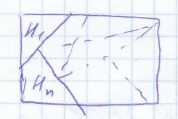
\includegraphics[scale=2.0]{full_group}}
	\caption{Полная группа}
\end{figure}

Замечание - события $H_{i}, i = \overline{1, n}$ часто называются гипотезами.\\

\subsection{Доказать теорему (формулу) полной вероятности и формулу Байеса}
Формула полной вероятности (теорема полной вероятности):\\
Пусть:\\
1) $H_{1}, ... H_{n}$ - полная группа событий\\
2) $P(H_{i}) > 0, i = \overline{1, n}$\\

Тогда $P(A) = P(A|H_{1})P(H_{1}) + ... + P(A|H_{n})P(H_{n})$ - формула полной вероятности\\

Доказательство:\\
1) $A = A \Omega = A (H_{1} + ... + H_{n}) = A H_{1} + ... + A H_{n}$\\
\begin{figure}[H]
	\center{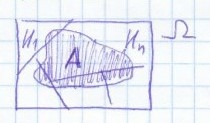
\includegraphics[scale=2.0]{full_group_prove}}
	\caption{Полная группа и событие A}
\end{figure}
2) $P(A) = P(A H_{1} + ... + A H_{n}) = | H_{i} H_{j} = \varnothing, i \neq j \Rightarrow (A H_{i}) (A H_{j}) = H_{i} H_{j} = \varnothing $ (так как события $H_{i}, H_{j}$ фиксированные и не пересекаются, то произведения A с каждым из этих событий так же не будут пересекаться, следовательно их произведение будет равно $\varnothing) | = P(A H_{i}) + ... + P(A H_{n}) = |$по формуле умножения вероятностей$| = P(A|H_{1})P(H_{1}) + ... + P(A|H_{n})P(H_{n})$\\
\\

Формула Байеса:\\
Пусть:\\
1) выполнены все условия из теоремы о формуле полной вероятности\\
2) P(A) > 0\\

Тогда $P(H_{i}|A) = \frac{P(A|H_{i})P(H_{i})}{P(A|H_{1})P(H_{1}) + ... + P(A|H_{n})P(H_{n})}, i = \overline{1, n}$\\

Доказательство:\\
$P(H_{i}|A) = \frac{P(A H_{i})}{P(A)} = \frac{P(A|H_{i})P(H_{i})}{P(A|H_{1})P(H_{1}) + ... + P(A|H_{n})P(H_{n})}, i = \overline{1, n}$ - по формуле полной вероятности и теореме умножения вероятностей\\

\subsection{Понятия априорной и апостериорной вероятностей}
Априорная вероятность - вероятность $P(H_{i})$ гипотез $H_{i}$ до проведения опыта.\\
Апостериорная вероятность - вероятность $P(H_{i}|A)$ гипотез $H_{i}$, уточнённых в результате опыта, исходом которого стало обытие A.\\

\section{Сформулировать определение схемы испытаний Бернулли. Доказать формулу для вычисления вероятности реализации ровно k успехов из n испытаний по схеме Бернулли. Доказать следствия из этой формулы}

\subsection{Сформулировать определение схемы испытаний Бернулли}

Определение схемы испытаний Бернулли (биноминальной схемой) - схемой испытаний Бернулли или биноминальной схемой называют серию экспериментов в каждом из которых возможны лишь два исхода — «успех» и «неудача», при этом успех в каждом испытании происходит с вероятностью $p \in \{0, 1\}$, а неудача с вероятностью $q = 1 - p$. Данная серия экспериментов должлна обладать следующими свойствами:\\
1) все испытания независимы, то есть исход $k$-го испытания не зависит от исходов испытаний с номерами $1, ..., k-1$\\
2) вероятноть осуществления успеха во всех испытаниях неизменна\\

\subsection{Доказать формулу для вычисления вероятности реализации ровно k успехов из n испытаний по схеме Бернулли. Доказать следствия из этой формулы}
Формула для вычисления вероятности реализации ровно k успехов из n испытаний по схеме Бернулли (Формула Бернулли) - $P_{n}(k) = C^{k}_{n} p^{k} q^{n - k}, k = 0, 1, ... n$, $(C^{k}_{n} = \frac{n!}{k! (n - k)!})$\\

Доказательство формулы для вычисления вероятности реализации ровно k успехов из n испытаний по схеме Бернулли:\\
1) Результат серии испытаний из n испытаний будем описывать кортежем $\omega = (x_{1}, ... x_{n})$,\\
где:\\
\begin{equation}
x_{i} = 
 \begin{cases}
   1 & \text{если в i-м испытании удача}\\
   0 & \text{иначе}\\
 \end{cases}
\end{equation}
2) A = \{ произошло ровно k успехов \}, тогда A = \{$\omega$ : в которых ровно k единиц\}\\
Число исходов в A равно количеству способов поставить в котреже $\omega$ ровно k единиц, что в свою очередь равно числу способов выбрать в $\omega$ k позиций для расстановки единиц = $C^{k}_{n}$\\
3) для каждого $\omega = (x_{1}, ... x_{n}) \in A$:\\
$P(\omega) = P(x_{1} ... x_{n}) = P($\{в первом испытании результат $x_{1}$\}$\cdot$ ... $\cdot$\{в n-ном испытании результат $x_{n}$\}) (так как испытания независимые, то) = P(\{в первом испытании результат $x_{1}$\})$\cdot$ ... $\cdot$P(\{в n-ном испытании результат $x_{n}$\}) (ровно k успехов и n неудач) = $p^{k} q^{n - k}$\\
4) так как $|A| = C^{k}_{n}$, то $P(A) = C^{k}_{n} p^{k} q^{n - k}$\\

Следствия из формулы для вычисления вероятности реализации ровно k успехов из n испытаний по схеме Бернулли:\\
Следствие 1: вероятность того, что число успехов в серии из n испытаний схемы Бернулли не менее $k_{1}$ и не более $k_{2}$:\\
$P_{n}(k_{1} \leqslant k \leqslant k_{2}) = \sum\limits^{k_{2}}_{i = k_{1}} C^{i}_{n} p^{i} q^{n - i}, k_{1} \leqslant k_{2}$\\
Доказательство:\\
Пусть A = \{ произошло $\geqslant k_{1}$ и $\leqslant k_{2}$ успехов\}\\
Тогда $A = A_{k_{1}} + ... + A_{k_{2}}$, где $A_{i}$ = \{произошло ровно i успехов\}, $i = \overline{k_{1}; k_{2}}\\
$P(A) = P($\sum\limits^{k_{2}}_{i = k_{1}} A_{i}$) = (так как $A_{i}$ несовместны) = $\sum\limits^{k_{2}}_{i = k_{1}} P(A_{i}) = \sum\limits^{k_{2}}_{i = k_{1}} C^{i}_{n} p^{i} q^{n - i}$\\

Следствие 2: вероятность того. что в серии из n испытаний по схеме Бернулли произойдёт хотя бы один успех, можно найти по формуле: $P(k \geqslant 1) = 1 - q^{n}$\\
Доказательство:\\
$P_{n}(k \geqslant 1) = 1$ - P \{в серии из n испытаний будет 0 успехов\} = $1 - P_{n}(0) = 1 - q^{n}$\\

\chapter{Случайные величины}
\section{Сформулировать определение случайной величины и функции распределения вероятностей случайной величины. Доказать свойства функции распределения}
\subsection{Сформулировать определение случайной величины и функции распределения вероятностей случайной величины}
Определение случайной величины - случайной величиной называют скалярную функцию $X(\omega)$ такую, что для $\forall x \in \mathcal{R}$ множество элементарных исходов $\{ \omega : X(\omega) < x \}$ является событием.\\

Определение функции распределения вероятностей - функцей распределения вероятностей случайной величины X называют функцию $F(x)$, значение которой в точке $x$ равно вероятности события $\{X < x\}$, то есть события, состоящего из тех и только тех элементарных исходов $\omega$, для которых $X(\omega) < x$: $F(x) = P(X < x)$.\\

\subsection{Доказать свойства функции распределения}
Свойства функции распределения:\\
1) $0 \leqslant F(x) \leqslant 1$\\
Доказательство:\\
F(x) = P\{X < x\} $\Rightarrow 0 \leqslant F(x) \leqslant 1$\\
2) если $x_{1} \leqslant x_{2}$, то $F(x_{1}) \leqslant F(x_{2})$, то есть F(x) - неубывающая функция\\ 
Доказательство:\\
$A_{1} = \{ X < x_{1}\}$\\
$A_{2} = \{ X < x_{2}\}$\\
так как $x_{1} \leqslant x_{2}$, то $A_{1} \leqslant A_{2}$. По свойству вероятности $P(A_{1}) \leqslant P(A_{2})$, $F(x_{1}) \leqslant F(x_{2})$\\
3) $\lim\limits_{x \rightarrow -\infty} F(x) = 0$ и $\lim\limits_{x \rightarrow +\infty} F(x) = 1$\\
Доказательство:\\
a) Докажем, что $\lim\limits_{x \rightarrow +\infty} F(x) = 1$\\
рассмотрим последовательность $x_{1}, x_{2} ... x_{n}$, такую, что:\\
1. $x_{1} \leqslant x_{2} \leqslant x_{3} \leqslant ... \leqslant x_{n}$\\
2. $x_{n} 	\rightarrow +\infty, n \rightarrow \infty$\\
Рассмотрим последовательность событий:\\
$A_{n} = \{X < x_{n}\}, n \geqslant 1$\\
Тогда $A_{n}, n = 1, 2, ...$ - возрастающая последовательность, так как $A_{i} \leqslant A_{i+1}, i = 1, 2, ...$\\
В соответствие с аксиомой непрерывности:\\
$\lim\limits_{n \rightarrow +\infty} P\{A_{n}\} = P \{ \cup^{\infty}_{n = 1} A_{n} \} = P \{ X < +\infty \}$ (то, что X меньше бесконечности - достоверное событие, следовательно происходит всегда) = 1\\
Так как $P\{A_{n}\} = P \{ X < x_{n} \} = F(x_{n})$, то тогда по определению предела функции по Гейне: $\lim\limits_{x \rightarrow +\infty} F(x_{n}) = 1$\\
$\lim\limits_{x \rightarrow +\infty} F(x) = 1$\\
б) равенство $\lim\limits_{x \rightarrow -\infty} F(x) = 0$ доказывается аналогично\\
4) $P\{x_{1} \leqslant x < x_{2}\} = F(x_{2}) - F(x_{1})$\\
Доказательство:\\
рассмотрим три события:\\
\begin{figure}[H]
	\center{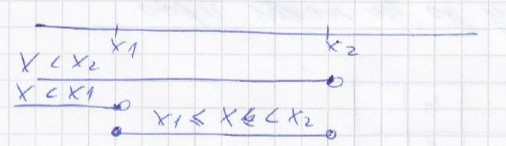
\includegraphics[scale=1.6]{three_cases}}
	\caption{Три события}
\end{figure}
5) $\lim\limits_{x \rightarrow x_{0}} F(x) = F(x_{0})$, то есть F(x) - непрерывна слева в каждой точке $x \in R$\\
Доказательство:\\
Рассмотрим последовательность $x_{1}, x_{2}, ..., x_{n}, ..., $, такую, что:\\
1. $x_{1} \leqslant x_{2} \leqslant ... \leqslant x_{n} \leqslant ... < x_{0}$\\
2. $x_{n} \rightarrow x_{0}$\\
Тогда $A_{n} = \{ X < x_{n} \}$ - неубывающая последовательность событий, $\lim\limits_{n \rightarrow \infty} P \{A_{n}\}$ = (по аксиоме непрерывности) = $P \{ \cup^{\infty}_{n = 1} A_{n} \} = P \{ X < x_{0} \} = F(x_{0})$, тогда $\lim\limits_{n \rightarrow \infty}  P \{A_{n}\} = \lim\limits_{n \rightarrow \infty}  F \{x_{n}\}$, по определению предела функции по Гейне $\lim\limits_{x \rightarrow x_{0}-} F(x) = F(x_{0})$\\

\section{Сформулировать определение случайной величины и функции распределения вероятностей случайной величины. Сформулировать определение дискретной и непрерывной случайной величины. Доказать свойства плотности распределения вероятностей непрерывной случайной величины}
\subsection{Сформулировать определение случайной величины и функции распределения вероятностей случайной величины}
Рассмотрено в пункте 2.1.1\\
\subsection{Сформулировать определение дискретной и непрерывной случайной величины}
Определение дискретной случайной величины - случайная величина X называется дискретной, если множество её значений конечно или счётно.

Определение непрерывной случайной величины - случайная величина X называется непрерывной, если $\exists f(x)$, такая, что функция распределения случайной величины X может быть представлена в виде $F(x) = \int_{-\infty}^{x} f(t) dt$\\
\begin{figure}[H]
	\center{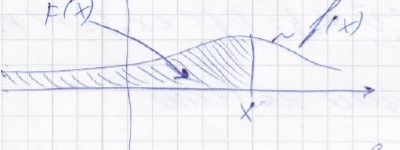
\includegraphics[scale=2.0]{integral_1}}
	\caption{Отношение F(x) и f(x)}
\end{figure}

\subsection{Доказать свойства плотности распределения вероятностей непрерывной случайной величины}
Свойства функции плотности распределения вероятностей:\\
1) $f(x) \geqslant 0, x \in R$\\

Доказательство:\\
$f(x) = F'(x)$, так как F(x) - неубывающая функция, то производная $F'(x) \geqslant 0 \Rightarrow f(x) \geqslant 0$\\

2) $P \{x_{1} \leqslant X < x_{2} \} = \int\limits_{x_{1}}^{x_{2}} f(x) dx$\\

Доказательство:\\
По свойству функции распределения $P \{x_{1} \leqslant X < x_{2} \} = F(x_{2}) - F(x_{1})$, так как F(x) - первообразная для f(x), то по формуле Ньютона-Лейбница $F(x_{2}) - F(x_{1}) = \int\limits_{x_{1}}^{x_{2}} f(x) dx$\\

3) $\int\limits_{-\infty}^{+\infty} f(x) dx = 1$\\

Доказательство:\\
$\int\limits_{-\infty}^{+\infty} f(x) dx = $ по свойству 2 $ = F(+\infty) - F(-\infty) = 1 - 0 = 1$\\

4) при малых $\Delta x, P \{x_{0} \leqslant X < x_{0} + \Delta x\} \approx f(x_{0}) \Delta x$\\

Доказательство:\\
$P \{x_{0} \leqslant X < x_{0} + \Delta x\} = F(x_{2}) - F(x_{1}) = $(так как f непрерывна, то воспольнуемся теоремой Лагранжа $\frac{f(b) - f(a)}{b - a} = f'(x_{0})$, где $x_{0}$ - некая точка в отрезке от a до b)$ = f(\xi)$, где $\xi \in (x_{0}, x_{0} + \Delta x)$\\
\begin{figure}[H]
	\center{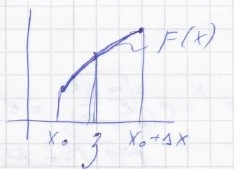
\includegraphics[scale=2.0]{x_0}}
	\caption{Функция F(x) и $\xi$}
\end{figure}
Так как $\Delta x$, "мало"  (стремится к 0), а f непрерывна, то $f(\xi) \approx f(x_{0})$, следовательно, $P \{x_{0} \leqslant X < x_{0} + \Delta x\} \approx f(x_{0}) \Delta x$\\

5) если X - непрерывная случайная величина, то для любого наперёд заданного $x_{0}, P(X = x_{0}) = 0$\\

Доказательство:\\
$P\{X = x_{0}\} = \lim\limits_{\Delta x \rightarrow 0} P \{x_{0} \leqslant X < x_{0} + \Delta x\} = \lim\limits_{\Delta x \rightarrow 0} f(\xi) \Delta x, \xi \in (x_{0}, x_{0} + \Delta x) = $ так как f(x) нерперывна, следовательно f($\xi$) ограничена = [органиченная $\cdot$ бесконечно малая] = 0\\

\section{Сформулировать определение нормальной случайной величины, геометрический смысл параметров. Понятние стандартного нормального закона. Доказать фомулу вычисления вероятности попадания нормальной случайной величины в интервал}

\subsection{Сформулировать определение нормальной случайной величины, геометрический смысл параметров}
Определение нормальной случайной величины - нормальная случайная величина $X \sim N(m, \sigma^{2})$, говорят, что непрерывная случайная величина X имеет нормальное распределение (распределение Гаусса) с параметрами m и $\sigma^{2}$, если её плотность распределения имеет вид:\\
$f(x) = \frac{1}{\sqrt{2 \pi} \sigma} e^{-\frac{(x - m)^{2}}{2\sigma^{2}}}, x \in R$, где $\sigma > 0, m \in \mathcal{R}$\\
\begin{figure}[H]
	\center{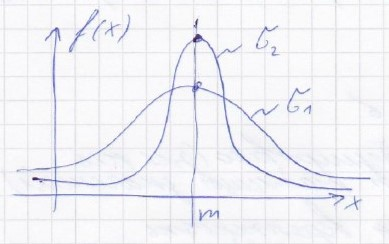
\includegraphics[scale=2.0]{normal}}
	\caption{Нормальное распределение}
\end{figure}

Геометрический смысл параметров нормального распределения - параметр m характеризует положение центра симметричности графика f(x). Параметр $\sigma$ отвечает за степень разброса значений случайной величины относительно среднего значения, чем больше $\sigma$, тем больше разброс.

\subsection{Понятние стандартного нормального закона}
Понятие стандартного нормального закона - если m = 0, $\sigma = 1$, то нормальная случайная величина $X \sim N(0, 1)$ называется стандартной нормальной величиной.

\subsection{Доказать фомулу вычисления вероятности попадания нормальной случайной величины в интервал}
Формула вычисления попадания вероятности нормальной случайной величины в интервал - если нормальная случайная величина не является стандартной, то попадание нормальной случайной величины в интервал вычисляется следующим образом:\\
$P(a \leqslant X < b) = \Phi(\frac{b - m}{\sigma}) - \Phi(\frac{a - m}{\sigma})$\\

Доказательство:\\
$P(a \leqslant X < b) = \frac{1}{\sqrt{2\pi} \sigma} \int\limits_{a}^{b} e^{-\frac{(x - m)^2}{2 \sigma^2}} dx = $ делаем замену: $t  = \frac{x -m}{\sigma}, dt = \frac{1}{\sigma} dx, x = a \Rightarrow t = \frac{a - m}{\sigma}, x = b \Rightarrow t = \frac{b - m}{\sigma} = \frac{\sigma}{\sqrt{2 \pi} \sigma} \int\limits^{\frac{b - m}{\sigma}}_{\frac{a - m}{\sigma}} e^{-\frac{t^{2}}{2}} dt = \frac{1}{\sqrt{2 \pi}} \int\limits^{\frac{b - m}{\sigma}}_{\frac{a - m}{\sigma}} e^{-\frac{t^{2}}{2}} dt = $ вероятность того, что стандартная нормальная случайная величина попала в промежуток $[\frac{a - m}{\sigma}, \frac{b  - m}{\sigma}) = \Phi(\frac{b - m}{\sigma}) - \Phi(\frac{a - m}{\sigma})$\\

\section{Сформулировать определение случайного вектора и функции распределения вероятностей случайного вектора. Сформулировать свойства функции распределения двумерного случайного вектора. Доказать предельные свойства}

\subsection{Сформулировать определение случайного вектора и функции распределения вероятностей случайного вектора}

Определение случайного вектора:\\
Пусть $(\Omega, \mathcal{B}, P)$ - вероятностное пространство. $X_{1}(\omega), ... , X_{n}(\omega)$ - случайные величины, заданные на этом вероятностном пространстве.\\
Тогда n-мерным случайным вектором называют кортеж $X_{1}(\omega), ... , X_{n}(\omega)$.\\

Определение функции распределения вероятностей случайного вектора:\\
Пусть $(\Omega, \mathcal{B}, P)$ - вероятностное пространство. $X_{1}(\omega), ... , X_{n}(\omega)$ - случайные величины, заданные на этом вероятностном пространстве.\\
Тогда функцией распределение вероятностей n-мерного случайного вектора $(X_{1}, ... X_{n})$ называется отображение $F : R^{n} \rightarrow R$, которое определено условием:\\
$F(x_{1}, ... x_{n}) - P(X_{1} < x_{1}, ... X_{n} < x_{n})$\\

\subsection{Сформулировать свойства функции распределения двумерного случайного вектора}
1) $0 \leqslant F(x_{1}, x_{2}) \leqslant 1$\\
2) при фиксированном $X_{2}$ функция $F(x_{1}, x_{2})$ является неубывающей функцией от $X_{1}$, при фиксированном $X_{1}$ функция $F(x_{1}, x_{2})$ является неубывающей функцией от $X_{2}$\\
3) $\lim\limits_{x_{2} \rightarrow -\infty} F(x_{1}, x_{2}) = 0$, $\lim\limits_{x_{1} \rightarrow -\infty} F(x_{1}, x_{2}) = 0$\\
4) $\lim\limits_{x_{1}, x_{2} \rightarrow +\infty} F(x_{1}, x_{2}) = 1$\\
5) $\lim\limits_{x_{2} \rightarrow +\infty} F(x_{1}, x_{2}) = F_{X_1} (x_{1})$, $\lim\limits_{x_{1} \rightarrow +\infty} F(x_{1}, x_{2}) =  F_{X_2} (x_{2})$\\
6) $P(a_{1} \leqslant X_{1} < b_{1}, a_{2} \leqslant X_{2} < b_{2}) = F(b_{1}, b_{2}) - F(a_{1}, b_{2}) - F(b_{1}, a_{2}) + F(a_{1}, a_{2})$\\
7) при фиксированном $X_{2}, F(x_{1}, x_{2})$ как функция $X_{1}$ является непрерывной слева во всех точках, при фиксированном $X_{1}, F(x_{1}, x_{2})$ как функция $X_{2}$ является непрерывной слева во всех точках\\

\subsection{Доказать предельные свойства}
1) $0 \leqslant F(x_{1}, x_{2}) \leqslant 1$\\
Доказательство:\\
Так как $F(x_{1}, x_{2}) = P(X_{1} < x_{1}, X_{2} < x_{2})$, то по свойствам вероятности $0 \leqslant F(x_{1}, x_{2}) \leqslant 1$\\

2) при фиксированном $X_{2}$ функция $F(x_{1}, x_{2})$ является неубывающей функцией от $X_{1}$, при фиксированном $X_{1}$ функция $F(x_{1}, x_{2})$ является неубывающей функцией от $X_{2}$\\
Доказательство:\\
a) Зафиксируем $X_{2}$, $F(x_{1}, x_{2}) = P(X_{1} < x_{1}, X_{2} < x_{2})$.\\
Тогда путь у нас есть два события:\\
$A_{1} = \{X_{1} < x_{1}^{'}, X_{2} < x_{2}\}$\\
$A_{2} = \{X_{1} < x_{2}^{'}, X_{2} < x_{2}\}$\\
и $x_{1}^{'} \leqslant x_{2}^{'}$\\
Тогда $A_{1} \leqslant A_{2}$, по свойству вероятности $P(A_{1}) \leqslant P(A_{2}) \Rightarrow F(x_{1}^{'}, x_{2}) \leqslant F(x_{2}^{'}, x_{2})$\\

3) $\lim\limits_{x_{2} \rightarrow -\infty} F(x_{1}, x_{2}) = 0$, $\lim\limits_{x_{1} \rightarrow -\infty} F(x_{1}, x_{2}) = 0$\\
Доказательство:\\
a) $\lim\limits_{x_{2} \rightarrow -\infty} F(x_{1}, x_{2}) = 0$\\
Рассмотрим событие $\{X_{1} < x_{1}\} \cdot \{X_{2} < -\infty\} \Rightarrow \{X_{1} < x_{1}\} \cdot \{X_{2} < -\infty\}$ - невозможно, так как $X_{2} < -\infty$ - невозможное событие, следовательно $F(X_{1}, -\infty) = P(X_{1} < x_{1}, X_{2} < -\infty) = 0$, тогда $\lim\limits_{x_{2} \rightarrow -\infty} F(x_{1}, x_{2}) = F(x_{1}, -\infty) = 0$\\
б) $\lim\limits_{x_{1} \rightarrow -\infty} F(x_{1}, x_{2}) = 0$ - доказывается аналогично a)\\

4) $\lim\limits_{x_{1}, x_{2} \rightarrow +\infty} F(x_{1}, x_{2}) = 1$\\
Доказательство:\\
рассмотрим последовательности $x_{1}^{1}, x_{2}^{1} ... x_{n}^{1}$ и $x_{1}^{2}, x_{2}^{2} ... x_{n}^{2}$, такие, что для $\forall i \in \{1, 2\}$:\\
1. $x_{1}^{i} \leqslant x_{2}^{i} \leqslant x_{3}^{i} \leqslant ... \leqslant x_{n}^{i}$\\
2. $x_{n}^{i} \rightarrow +\infty, n \rightarrow \infty$\\
Рассмотрим последовательность событий:\\
$A_{n} = \{X_{1} < x_{n}^{1}, X_{2} < x_{n}^{2}\}, n \geqslant 1$\\
Тогда $A_{n}, n = 1, 2, ...$ - возрастающая последовательность, так как $A_{i} \leqslant A_{i+1}, i = 1, 2, ...$\\
В соответствие с аксиомой непрерывности:\\
$\lim\limits_{n \rightarrow +\infty} P\{A_{n}\} = P \{ \cup^{\infty}_{n = 1} A_{n} \} = P \{ X_{1} < +\infty, X_{2} < +\infty \}$ ($X_{1} < +\infty, X_{2} < +\infty$ - достоверные события) = 1\\
Так как $P\{A_{n}\} = P \{X_{1} <  x_{n}^{1}, X_{2} < x_{n}^{2}\} = F( x_{n}^{1},  x_{n}^{2})$, то тогда по определению предела функции по Гейне: $\lim\limits_{x_{1}, x_{2} \rightarrow +\infty} F(x_{1}, x_{2}) = 1$\\

либо:

Рассмотрим события $\{X_{1} < +\infty\}, \{X_{1} < +\infty\}$, данные события являются достоверными, также, как и их пересечение. Тогда так как $P(X_{1} < +\infty, X_{2} < +\infty) = 1, \lim\limits_{x_{1}, x_{2} \rightarrow +\infty} F(x_{1}, x_{2})  = F(+\infty, +\infty) = P(X_{1} < +\infty, X_{2} < +\infty) = 1$\\

5) $\lim\limits_{x_{2} \rightarrow +\infty} F(x_{1}, x_{2}) = F_{X_1} (x_{1})$, $\lim\limits_{x_{1} \rightarrow +\infty} F(x_{1}, x_{2}) =  F_{X_2} (x_{2})$\\
Доказательство:\\
Докажем, что $\lim\limits_{x_{2} \rightarrow +\infty} F(x_{1}, x_{2}) = F_{X_1} (x_{1})$:\\
Событие $\{X_{2} < +\infty\}$ является достоверным $\Rightarrow \{X_{1} < x_{1}\} \cdot \{X_{2} < +\infty\} = \{X_{1} < x_{1}\}$\\
Тогда $F(x_{1}, +\infty) = P(X_{1} < x_{2}) = F_{X_{1}}(x_{1})$\\
Для $X_{2}$ доказывается аналогично.\\

\section{Сформулировать определение случайного вектора и функции распределения вероятностей случайного вектора. Сформулировать свойства функции распределения двумерного случайного вектора. Доказать формулу для вычисления $P(a_{1} \leqslant X_{1} < b_{1}, a_{2} \leqslant X_{2} < b_{2})$}
\subsection{Сформулировать определение случайного вектора и функции распределения вероятностей случайного вектора}
Рассмотрено в пункте 2.4.1
\subsection{Сформулировать свойства функции распределения двумерного случайного вектора}
Рассмотрено в пункте 2.4.2
\subsection{Доказать формулу для вычисления $P(a_{1} \leqslant X_{1} < b_{1}, a_{2} \leqslant X_{2} < b_{2})$}
\begin{figure}[H]
	\center{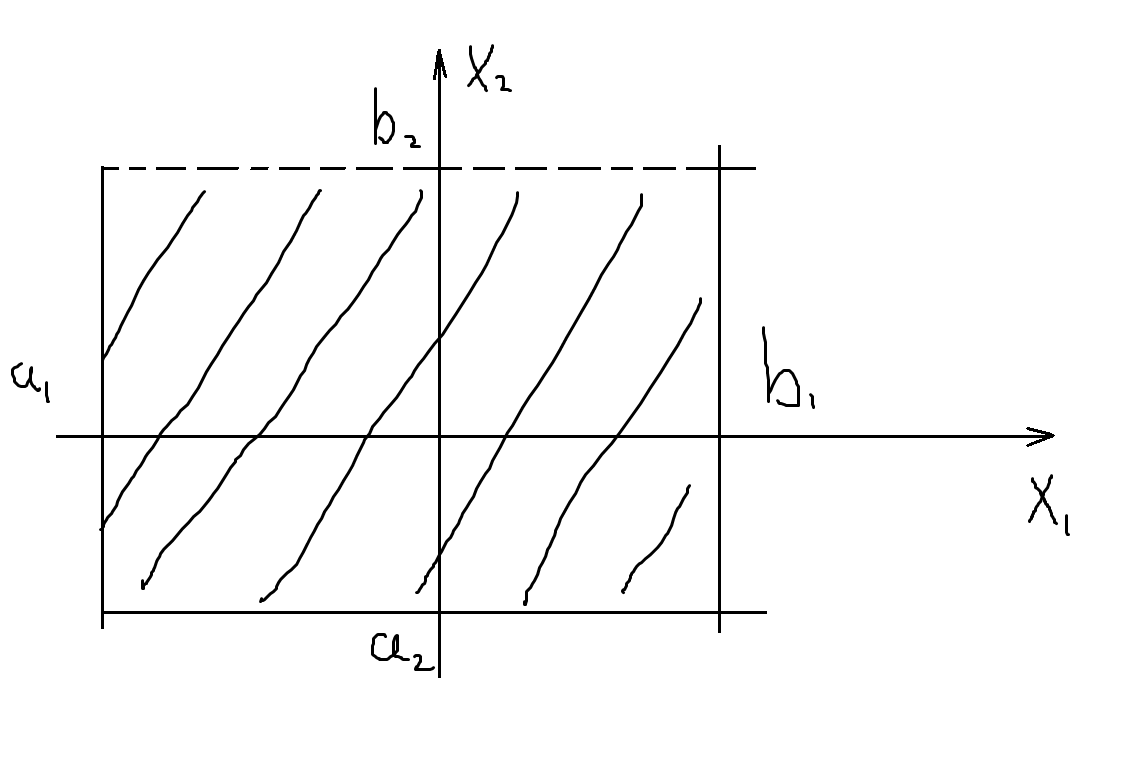
\includegraphics[scale=0.2]{exp_1}}
	\caption{Нормальное распределение}
\end{figure}
a) Найдём вероятность того, что случайный вектор попадёт в полосу $\{X_{1} < x_{1}, a_{2} \leqslant X_{2} < b_{2}\}$\\
$F(x_{1}, b_{2}) = P(X_{1} < x_{1}, X_{2} < b_{2})$ - область под $b_{2}$ и слева от $a_{1} (x_{1})$\\
$F(x_{1}, a_{2}) = P(X_{1} < x_{1}, X_{2} < a_{2})$ - область под $a_{2}$ и слева от $a_{1} (x_{1})$\\
$P(X_{1} < x_{1}, a_{2} \leqslant  X_{2} < b_{2}) = F(x_{1}, b_{2}) - F(x_{1}, a_{2})$\\
б) по полученной в a) формуле $F(b_{1}, b_{2}) - F(b_{1}, a_{2})$ - область область под $b_{2}$, слева от $a_{1}$ и выше $a_{2}$\\
$F(a_{1}, b_{2}) - F(a_{1}, a_{2})$ - область между $b_{2}, a_{2}$ и слева от $a_{1}$\\
Тогда  $P(a_{1} \leqslant X_{1} < b_{1}, a_{2} \leqslant X_{2} < b_{2}) = (P(X, Y)$ принадлежащей области слева от $b_{1}$ и ниже $b_{2}$) - (P(X, Y) принадлежащей области слева от $a_{1}$ и ниже $b_{2}$ и области слева от $b_{1}$ и ниже $a_{2}$) = $F(b_{1}, b_{2}) - F(b_{1}, a_{2}) - F(a_{1}, b_{2}) + F(a_{1}, a_{2})$\\

\section{Сформулировать определение случайного вектора и функции распределения вероятностей случайного вектора. Сформулировать определение непрерывного случайного вектора и доказать свойства плотности распределения вероятностей для двумерного случайного вектора}

\subsection{Сформулировать определение случайного вектора и функции распределения вероятностей случайного вектора}
Рассмотрено в пункте 2.4.1

\subsection{Сформулировать определение непрерывного случайного вектора и доказать свойства плотности распределения вероятностей для двумерного случайного вектора}
Определение непрерывного случайного вектора - случайный вектор $(X_{1}, ... X_{n})$ называется непрерывным, если $\exists f(x_{1}, ... x_{n})$ такая, что:\\
$F(X_{1}, ... F_{n}) = \int\limits^{x_{1}}_{-\infty} dt_{1} \int\limits^{x_{2}}_{-\infty} dt_{2} ... \int\limits^{x_{n}}_{-\infty} f(t_{1}, ... t_{n}) dt_{n}$\\

При этом:\\
1) функция $f(x_{1}, ... x_{n})$ называется плотностью распределения вероятностей случайного вектора $(x_{1}, ... x_{n})$\\
2) предполагается, что указанные несобственные интегралы сходятся для всех $(x_{1}, ... x_{n}) \in R^{n}$\\

\subsection{Доказать свойства плотности распределения вероятностей для двумерного случайного вектора}
1)$f(x_{1}, x_{2}) \geqslant 0$\\

Доказательство:\\
Так как $f(x_{1}, x_{2})$ - первообразная неубывающей функции распределения случайного вектора $F(X_{1}, X_{2})$, то по свойствам первообразной $f(x_{1}, x_{2}) \geqslant 0$\\

2)$P(a_{1} \leqslant X_{1} < b, a_{2} \leqslant X_{2} < b_{2}) = \int\limits^{b_{1}}_{a_{1}} dx_{1} \int\limits^{b_{2}}_{a_{2}} f(x_{1}, x_{2}) dx_{2}$

Доказательство:\\
$P(a_{1} \leqslant X_{1} < b_{1}, a_{2} \leqslant X_{2} < b_{2}) =F(b_{1}, b_{2}) - F(a_{1}, b_{2}) - F(b_{1}, a_{2}) + F(a_{1}, a_{2}) = (F(b_{1}, b_{2}) - F(a_{1}, b_{2})) - (F(b_{1}, a_{2}) - F(a_{1}, a_{2})) = \int\limits^{b_{1}}_{a_{1}} dx_{1} \int\limits^{b_{2}}_{a_{2}} f(x_{1}, x_{2}) dx_{2}$\\

3)$\iint\limits_{R^{2}} f(x_{1}, x_{2}) dx_{1} dx_{2}$\\

Доказательство:\\
$\iint\limits_{R^{2}} f(x_{1}, x_{2}) dx_{1} dx_{2} = P(-\infty \leqslant X_{1} < +\infty , -\infty \leqslant X_{2} < +\infty) = F(+\infty, +\infty) - F(+\infty, -\infty)  - F(-\infty, +\infty) + F(-\infty, -\infty) = $ по свойствам функции распределения $ = 1 + 0 + 0 + 0 = 1$\\

4)$P(a_{1} \leqslant X_{1} < a_{1} + \Delta x_{1}, a_{2} \leqslant X_{2} < a_{2} + \Delta x_{2}) \cong f(a_{1}, a_{2}) \cdot \Delta x_{1} \cdot \Delta x_{2}$, где $(a_{1}, a_{2})$ - точка непрерывной функции $f(x_{1}, x_{2})$\\

Доказательство:\\
$P(a_{1} \leqslant X_{1} < a_{1} + \Delta x_{1}, a_{2} \leqslant X_{2} < a_{2} + \Delta x_{2}) =  F(a_{1} + \Delta x_{1}, a_{2} + \Delta x_{2}) - F(a_{1}, a_{2} + \Delta x_{2}) - F(a_{1} + \Delta x_{1}, a_{2}) + F(a_{1}, a_{2}) = (F(a_{1} + \Delta x_{1}, a_{2} + \Delta x_{2}) - (F(a_{1}, a_{2} + \Delta x_{2})) - F(a_{1} + \Delta x_{1}, a_{2}) - F(a_{1}, a_{2}))$ (*)\\
Рассмотрим содержимое скобок, применив к каждой из них теорему Лагранжа:\\
$\frac{F(a_{1} + \Delta x_{1}, a_{2} + \Delta x_{2}) - F(a_{1}, a_{2} + \Delta x_{2})}{a_{1} + \Delta x_{1} - a_{1}} = \frac{\delta F(\xi_{1}, a_{2} + \Delta x_{2})}{\delta x_{1}}, \xi_{1} \in (a_{1}, a_{1} + \Delta x_{1})$\\
$\frac{F(a_{1} + \Delta x_{1}, a_{2}) - F(a_{1}, a_{2})}{a_{1} + \Delta x_{1} - a_{1}} = \frac{\delta F(\xi_{1}, a_{2})}{\delta x_{1}}, \xi_{1} \in (a_{1}, a_{1} + \Delta x_{1})$\\
Подставим получившееся в выражение (*):\\
$\frac{\frac{\delta F(\xi_{1}, a_{2} + \Delta x_{2})}{\delta x_{1}} - \frac{\delta F(\xi_{1}, a_{2})}{\delta x_{1}}}{a_{2} + \Delta x_{2} - a_{2}} = f(\xi_{1}, \xi_{2}), \xi_{2} \in (a_{2}, a_{2} + \Delta x_{2})$\\
$\frac{(F(a_{1} + \Delta x_{1}, a_{2} + \Delta x_{2}) - F(a_{1}, a_{2} + \Delta x_{2})) - (F(a_{1} + \Delta x_{1}, a_{2}) - F(a_{1}, a_{2}))}{\Delta x_{1}}  = f(\xi_{1}, \xi_{2}) \Delta x_{2}$\\
$(F(a_{1} + \Delta x_{1}, a_{2} + \Delta x_{2}) - F(a_{1}, a_{2} + \Delta x_{2})) - (F(a_{1} + \Delta x_{1}, a_{2}) - F(a_{1}, a_{2})) = f(\xi_{1}, \xi_{2})\Delta x_{1}  \Delta x_{2}$\\
Следовательно:\\
$P(a_{1} \leqslant X_{1} < a_{1} + \Delta x_{1}, a_{2} \leqslant X_{2} < a_{2} + \Delta x_{2}) =  f(\xi_{1}, \xi_{2})\Delta x_{1}  \Delta x_{2}, \xi_{1} \in (a_{1}, a_{1} + \Delta x_{1}), \xi_{2} \in (a_{2}, a_{2} + \Delta x_{2})$\\
При $\Delta x_{1} \rightarrow 0, \Delta x_{2} \rightarrow 0$:\\
$P(a_{1} \leqslant X_{1} < a_{1} + \Delta x_{1}, a_{2} \leqslant X_{2} < a_{2} + \Delta x_{2}) \cong f(a_{1}, a_{2}) \cdot \Delta x_{1} \cdot \Delta x_{2}$, где $(a_{1}, a_{2})$ - точка непрерывной функции $f(x_{1}, x_{2})$

5) для любого наперёд заданого значения $(x_{1}^{\circ}, x_{2}^{\circ}), P((X_{1}, X_{2}) = (x_{1}^{\circ}, x_{2}^{\circ})) = 0$\\

Доказательство:\\
По свойству 4:\\
$P(a_{1} \leqslant X_{1} < a_{1} + \Delta x_{1}, a_{2} \leqslant X_{2} < a_{2} + \Delta x_{2}) =  f(\xi_{1}, \xi_{2}) \Delta x_{1} \Delta x_{2}, \xi_{1} \in (a_{1}, a_{1} + \Delta x_{1}), \xi_{2} \in (a_{2}, a_{2} + \Delta x_{2})$\\
При $\Delta x_{1} = 0, \Delta x_{2} = 0$:\\
$P((X_{1}, X_{2}) = (x_{1}^{\circ}, x_{2}^{\circ})) = f(\xi_{1}, \xi_{2}) \cdot 0 \cdot 0 = 0$\\

6) $P((X_{1}, X_{2}) \in D) = \iint\limits_{D} f(x_{1}, x_{2}) dx_{1} dx_{2}$\\

Доказательство:\\
Является обобщением свойства 2 для произвольной области.

7) $\int\limits_{-\infty}^{+\infty} f(x_{1}, x_{2}) dx_{2} = f_{X_{1}}(x_{1})$, $\int\limits_{-\infty}^{+\infty} f(x_{1}, x_{2}) dx_{1} = f_{X_{2}}(x_{2})$\\

Доказательство:\\
a) покажем, что $\int\limits_{-\infty}^{+\infty} f(x_{1}, x_{2}) dx_{2} = f_{X_{1}}(x_{1})$\\
$F_{X_{1}}(x_{1}) = F(x_{1}, +\infty) = $ по определению непрерывного случайного вектора $ = \int\limits^{x_{1}}_{-\infty} dt_{1} \int\limits^{+\infty}_{-\infty} f(t_{1}, t_{2}) dt_{2}$\\

Продиффернцируем обе части по $x_{1}$:\\
$f_{X_{1}}(x_{1}) = \frac{dF(x_{1})}{dx_{1}} = $ то теореме о производной интеграла с переменным пределом $ = \int\limits^{+\infty}_{-\infty} f(x_{1}, t_{2}) dt_{2}$\\
б) доказывается аналогично a)\\

\section{Сформулировать определение пары независимых случайных величин. Доказать свойства независимых случайных величин. Понятия попарно независимых случайных величин и случайных величин, независимых в совокупности}

\subsection{Сформулировать определение пары независимых случайных величин}
Определение пары независимых случайных величин - случайные величины X, Y называются независимыми, если $F(x, y) = F_{X}(x)F_{Y}(y)$, где F - совместная функция распределения случайного вектора (X, Y).

\subsection{Доказать свойства независимых случайных величин}
Свойства независимых случайных величин:\\
1) $\forall x, \forall y \in R$ события $\{X < x\}, и \{Y < y\}$  - независимые.\\
Доказательство:\\
$P(X < x, Y < y) = F(x, y) = F_{X}(x) F_{Y}(y) = P(X < x) P(Y < y) \Rightarrow P(X < x, Y < y) = P(X < y) P(Y < y) \Rightarrow $ события независимы.\\

2) $\forall x_{1}, x_{2}, \forall y_{1}, y_{2} \in R$ события $\{x_{1} \leqslant X < x_{2}\}, и \{y_{1} \leqslant Y < y_{2}\}$  - независимые.\\
Доказательство:\\
a) докажем необходимость $\Rightarrow$:\\
Пусть X, Y - независимые, тогда $F(X, Y) = F_{X}(x) F_{Y}(y)$\\
По свойсту двумерной функции распределения:
$P(x_{1} \leqslant X < x_{2}, y_{1} \leqslant Y < y_{2}) = F(x_{2}, y_{2}) - F(x_{1}, y_{2}) - F(x_{2}, y_{1}) + F(x_{1}, y_{2}) = F_{X}(x_{2})F_{Y}(y_{2}) - F_{X}(x_{1})F_{Y}(y_{2}) - F_{X}(x_{2})F_{Y}(y_{1}) + F_{X}(x_{1})F_{Y}(y_{1}) = [F_{X}(x_{2}) - F_{X}(y_{1})][F_{Y}(y_{2} - )F_{Y}(y_{1})] = $ по свойству функций распределения = $ P(x_{1} \leqslant X < x_{2}) P(y_{1} \leqslant Y < y_{2}) $, следовательно события $\{x_{1} \leqslant X < x_{2}\}$, $\{y_{1} \leqslant Y < y_{2}\}$ - независимы\\
б) доказательство достаточности:\\
Пусть для любых $x_{1}, x_{2}, y_{1}, y_{2}$ события $\{x_{1} \leqslant X < x_{2}\}$, $\{y_{1} \leqslant Y < y_{2}\}$ - независимы, тогда:\\
$F(x, y) = P(x_{1} \leqslant X < x_{2}, y_{1} \leqslant Y < y_{2}) = $ так как события независимы $ = P(x_{1} \leqslant X < x_{2}) P(y_{1} \leqslant Y < y_{2}) = F_{X}(x) F_{Y}(y)$\\

3) $\forall M_{1}, M_{2}$, события $\{X \in M_{1}\}$ и $\{Y \in M_{2}\}$ независимы, где $M_{1}, M_{2}$ - промежутки или объединения промежутков в R.\\
Доказательство:\\
Яляется обобщением свойств 1 и 2.\\

4) если X, Y - дискретные случайные величины, если X, Y - независимы $\Leftrightarrow P((X, Y) = (x_{i}, y_{j})) = P(X = x_{i})P(Y = y_{j})$ для всех i, j\\
Доказательство:\\
$P((X, Y) = (x_{i}, y_{j})) = P((X = x{i}) (Y = y_{j})) = P(X = x_{i})P(Y = y_{j})$\\

5) Если X, Y - непрерывные случайные величины, то если $f(x, y) = f_{X}(x)f_{Y}(y)$, где f(x, y) - совместная плотность распределения вектора (X, Y), $f_{X}, f_{Y}$ - маргинальные плотности распределения величин X, Y.\\ 
Доказательство:\\
a) необходимость\\
X, Y - независимы тогда $F(x, y) = F_{X}(x)F_{Y}(y)$\\
$f(x, y) = \frac{\delta^{2}F(x, y)}{\delta x \delta y} = \frac{\delta^{2}}{\delta x \delta y}[F_{X}(x)F_{Y}(y)] = [\frac{\delta}{\delta x} F_{X}(x)][\frac{\delta}{\delta y} F_{Y}(y)] = f_{X}(x)f_{Y}(y)$\\
б) достаточность\\
пусть $f(x, y) = f_{X}(x)f_{Y}(y)$ тогда $F(x, y) = \int\limits_{-\infty}^{x} dt_{1} \int\limits_{-\infty}^{y} f(t_{1}, t_{2}) dt_{2} = \int\limits_{-\infty}^{x} dt_{1} \int\limits_{-\infty}^{y} f_{X}(t_{1})f_{Y}(t_{2}) dt_{2} = \int\limits_{-\infty}^{x}  f_{X}(t_{1}) dt_{1} \int\limits_{-\infty}^{y} f_{Y}(t_{2}) dt_{2} = F_{X}(x)F_{Y}(y) \Rightarrow X,Y$ - независимы.

\subsection{Понятия попарно независимых случайных величин и случайных величин, независимых в совокупности}
Понятие попрано независимых случайных величин - случайные величины $X_{1}, ... X_{n}$, заданные на одном вероятностном пространстве называются попарно независимыми если для всех $i \neq j, X_{i}, X_{j}$ - независимые случайные величины.\\

Понятие случайных величин, независимых в совокупности - случайные величины $X_{1}, ... X_{n}$, заданные на одном вероятностном пространстве называются независимыми в совокупности, если $F(X_{1}, ..., X_{n}) = F_{X_{1}}(x_{1}) \cdot ... \cdot F_{X_{n}}(x_{n})$, где $F$ - совместная функция распределения случайного вектора $(X_{1}, ..., X_{n})$\\

$F_{X_{i}}(x_{i})$ - маргинальная фунция распределения компоненты случайного вектора.\\

\section{Понятие условнго распределения случайной величины. Сформулировать определение условного ряда распределения компоненты двумерного дискретного случайного вектора. Привести рассуждения, приводящие к такому определению. Сформулировать определение условной плосткости распределения компоненты двумерного непрерывного случайного вектора. Сформулировать критерии независимости случайных величин в терминах условных распределений}
\subsection{Понятие условного распределения случайной величины}
Понятие условного распределения случайной величины - условное распределение это распределение случайной величины при условии, что другая случайная величина приняла определённое значение.

\subsection{Сформулировать определение условного ряда распределения компоненты двумерного дискретного случайного вектора. Привести рассуждения, приводящие к такому определению}
Определение условного ряда распределения компоненты двумерного дискретного случайного вектора - пусть:\\
1) (X, Y) - дискретный случайный вектор\\
2) $X \in \{x_{1}, ..., x_{m}\}$, $Y \in \{y_{1}, ..., y_{n}\}$\\
3) Обозначим $P_{ij} = P((X, Y) = (x_{i}, y_{j}))$\\
Тогда если $Y = y_{j}$ то $P(X = x_{i}|Y = y_{i}) = \frac{P(X = x_{i}, Y = y_{j})}{P(Y = y_{j})} = \frac{P_{ij}}{\sum\limits^{m}_{i = 1}P_{ij}} = \frac{P_{ij}}{P_{Yj}}$\\
Тогда для дискретного двумерного случайного вектора (X, Y) условной вероятностью того, что случайный вектора X принимает значение $x_{i}$, при условии, что случайная величина Y приняла значение $y_{i}$ называется число $\Pi_{ij} = \frac{P_{ij}}{P_{Yj}}$\\

\subsection{Сформулировать определение условной плостности распределения компоненты двумерного непрерывного случайного вектора}
Условной плотностью распределения непрерывной случайной величины X при условии, что случайная величина Y приняла значение y называется $f_{X}(x | Y = y) = \frac{f(x, y)}{f_{Y}(y)}$\\

\subsection{Сформулировать критерии независимости случайных величин в терминах условных распределений}
Критерий независимости случайных величин в терминах условных распределений - пусть $(X, Y)$ - случайный вектор, тогда $X, Y$ - независимые тогда и только тогда, когда условное распределение случайной величины $X$, при условии $Y = y$, совпадает с безусловным распределением случайной величины $X$:\\
1)$F(x | Y = y) = F_{X}(x)$\\
или\\
$F(y | X = x) = F_{Y}(y)$\\
2)X, Y - непрерывные величины, тогда:\\
$f_{X}(x | Y = y) = f_{X}(x)$\\
или\\
$f_{Y}(y | X = x) = f_{Y}(y)$\\
3) X, Y - дискретные величины:\\
$P(X = x_{i} | Y = y_{j}) = P(X = x_{i})$\\
или\\
$P(Y = y_{j} | X = x_{i}) = P(Y = y_{j})$\\

\section{Понятие функции скалярной случайной величины. Доказать теорему о формуле для вычисления плотности $f_{Y}(y)$ случайной величины $Y  = \phi(X)$, если X - непрерывная случайная величина, а $\phi$ - монотонная непрерывно дифференируемая функция. Записать аналогичную формулу для кусочно-монотонной функции $\phi$}
\subsection{Понятие функции скалярной случайной величины}
Понятие функции скалярной случайной величины - пусть:\\
1) на вероятностном пространстве $(\Omega, \mathcal(B), P)$ задана $X = X(\omega)$ - некоторая случайная величина\\
2) $Y : R \rightarrow R$ - действительная функция, действительного аргумента x\\
Тогда случаную величину $Y(\omega) = Y(X(\omega)) $ - называют функцией $Y(X)$ скалярной случайной величины $X$\\
\subsection{Доказать теорему о формуле для вычисления плотности $f_{Y}(y)$ случайной величины $Y  = \phi(X)$, если X - непрерывная случайная величина, а $\phi$ - монотонная непрерывно дифференируемая функция}
Теорема о формуле для вычисления плотности $f_{Y}(y)$ случайной величины $Y  = \phi(X)$:\\
пусть:\\
1) X - непрерывная случайная величина\\
2) $f_{X}(x)$ - плотность распределения случайной величины X\\
3) $\phi : R \rightarrow R$ - монотонная функция, которая непрерывна и дифференцируема\\
4) $\psi$ - функция, обратная к $\phi$\\
5) $Y = \phi(X)$\\
Тогда Y - непрерывная случайная величина, плотность распределения которой:\\
$f_{Y}(y) = f_{X}(\psi(y))|\psi(y)'|$\\

Доказательство:\\
По определению функции распределения:\\
$F_{Y}(y) = P(Y < y) = P(\phi(x) < y)$\\
так как $\phi$ - монотонная, то $\exists$ обратная к ней функция $\phi^{-1} = \psi$\\
Событие \{$\phi(x) < y$\} = событие \{$X < \psi(y)$\} (если $\phi$ возврастающая функция)\\
иначе событие \{$\phi(x) < y$\} = событие \{$X > \psi(y)$\} (если $\phi$ возврастающая функция)\\
Тогда $F_{Y}(y) = P(X < \psi(y)) = F_{X}(\psi(y))$, если $\psi$ возрастающая, иначе\\
$F_{Y}(y) = P(X > \psi(y)) = 1 - F_{X}(\psi(y)) = 1 - F_{X}(\psi(y))$, если $\phi$ убывающая\\
Тогда $f_{Y}(y) = \frac{dF_{Y}(y)}{dy} = \frac{d}{dy}[F_{X}(\psi(y))] = F_{X}'(\psi(y))\psi'(y) = f_{X}(\psi(y))\psi'(y)$, если $\phi$ возрастает\\
$f_{Y}(y) = ... = -f_{X}(\psi(y))\psi'(y)$\\
Так как $f_{X} \geqslant 0$, знак $\psi'(y)$ зависит от возрастающей/убывающей фукнции $\phi$, то обе формулы можно объединить в:\\
$f_{Y}(y) = f_{X}(\psi(y))|\psi'(y)|$\\

\subsection{Записать аналогичную формулу для кусочно-монотонной функции $\phi$}
Теорема о формуле для вычисления плотности $f_{Y}(y)$ случайной величины $Y  = \phi(X)$ - кусочно монотонной функции:\\
пусть:\\
1) X - непрерывная случайная величина\\
2) $f_{X}(x)$ - плотность распределения X\\
3) $\phi: R \rightarrow R$ - имеет n интервалов монотонности $I_{1}, ..., I_{n}$\\
4) $\phi$ - непрерывная дифференцируемая функция\\
5) для данного $y \in R: x_{1}, ..., x_{n}$ - все решения уровня $\phi(x_{k}) = y, (k \leqslant n)$\\
6) $\psi_{1}(y), ..., \psi(y)$ - функции обратные к $\phi$ соответственно на тех интервалах монотонности, к которым принадлежат $x_{1}, ..., x_{n}$\\

Тогда для данного значения y:\\
$f_{Y}(y) = \sum\limits_{i = 1}^{n} f_{X}(\psi_{i}(y))|\psi_{i}'(y)|$\\

\section{Понятие функции скалярной функции случайного вектора. Обосновать формулу для вычисления функции распределения случайной величины Y, функционально зависящей от случайных величин $X_{1}, X_{2}$, если $(X_{1}, X_{2})$ - непрерывный случайный вектор. Доказать теорему о формуле свертки}
\subsection{Понятие скалярной функции случайного вектора}
Понятие функции скалярной функции случайного вектора - пусть:\\
1) $(X_{1}, X_{2})$ - случайный вектор, заданный на вероятностном пространстве $(\Omega, \mathcal{B}, P)$\\
2) $\phi : R^{2} \rightarrow R$ - действительная функция двух действительных переменных переменных\\
Тогда случайная величина $Y = \phi(X_{1}, X_{2})$ называется скалярной функцией случайного вектора.\\

\subsection{Обосновать формулу для вычисления функции распределения случайной величины Y, функционально зависящей от случайных величин $X_{1}, X_{2}$, если $(X_{1}, X_{2})$ - непрерывный случайный вектор}
Формула вычисления функции распределения случайной величины Y, функционально зависящей от случайных величин $X_{1}, X_{2}$, если $(X_{1}, X_{2})$ - непрерывный случайный вектор:\\
Если $(X_{1}, X_{2})$ - непрерывные случайный вектор, то:\\
$F_{Y} = \iint\limits_{\phi(x_{1}, x_{2}) < y} f(x_{1}, x_{2}) dx_{1} dx_{2}$, где $f(x_{1}, x_{2})$ - плотность распределения случайного вектора $(X_{1}, X_{2})$\\
Неравенство $\phi(x_{1}, x_{2}) < y$ обозначает \{$(x_{1}, x_{2}) : \phi(x_{1}, x_{2}) < y$\}\\

Замечание обоснавание формулы (*)\\
\begin{figure}[H]
	\center{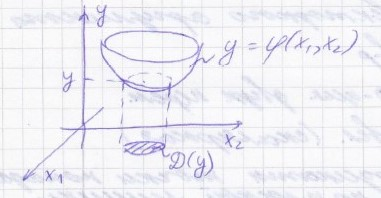
\includegraphics[scale=1.5]{memes}}
	\caption{Обоснование формулы}
\end{figure}

По определению $F_{Y}(y) = P(Y < y) = P(\phi(x_{1}, x_{2}) < y) = P((X_{1}, X_{2}) \in D(Y))$, таким образом:\\
$F_{Y}(y) = P((X_{1}, X_{2}) \in D(y))$ = по свойству плотности = $\iint\limits_{D(y)} f(x_{1}, x_{2}) dx_{1} dx_{2} = \iint\limits_{\phi(x_{1}, x_{2}) < y}f(x_{1}, x_{2}) dx_{1} dx_{2}$\\

\subsection{Доказать теорему о формуле свертки}
Теорема о формуле свёртки - пусть\\
1) $(X_{1}, X_{2})$ - непрерывный случайный вектор\\
2) $X_{1}, X_{2}$ - независимы\\
3) $Y = X_{1} + X_{2}$\\

Тогда $f_{Y}(y) = \int\limits_{-\infty}^{+\infty} f_{X_{1}}(x) f_{X_2}(y - x) dx$ - формула свёртки\\

Доказательство:\\
Так как $Y = Y(X_{1}, X_{2})$, где $Y(x_{1}, x_{2}) = x_{1} + x_{2}$, то:\\
$F_{Y}(y) = P(Y < y) = P(X_{1} + X_{2} < y) = \iint\limits_{x_{1} + x_{2} < y} f(x_{1}, x_{2}) dx_{1} dx_{2} = \int\limits_{-\infty}^{+\infty} dx_{1} \int\limits_{-\infty}^{y - x_{1}} f(x_{1}, x_{2}) dx_{2} = $ | так как $X_{1}, X_{2}$ - независимы, то $f(x_{1}, x_{2}) = f_{X_{1}}(x_{1})f_{X_{2}}(x_{2})$ |$ = \int\limits_{-\infty}^{+\infty} dx_{1} \int\limits_{-\infty}^{y - x{1}} f_{X_{1}}(x_{1}) f_{X_{2}}(x_{2}) dx_{2} = \int\limits^{+\infty}_{-\infty} f_{X_{1}}(x_{1}) dx_{1} \int\limits_{-\infty}^{y - x{1}} f_{X_{2}}(x_{2}) dx_{2} =  \int\limits^{+\infty}_{-\infty} f_{X_{1}}(x_{1}) F_{X_{2}} (y - x_{1}) dx_{1}$\\
Продиффренцируем обе части равенства:\\
$F_{Y}(y) = \int\limits_{-\infty}^{+\infty} f_{X_{1}}(x_{1}) F_{X_{2}}(y - x_{1}) dx_{1}$ по y:\\
$f_{Y}(y) = \int\limits_{-\infty}^{+\infty} f_{X_{1}}(x_{1}) f_{X_{2}}(y - x_{1}) dx_{1}$

\section{Сформулировать определение математического ожидания для дискретной и непрерывных случайных величин. Механический смысл математического ожидания. Доказать свойства математического ожидания. Записать формулы для вычисления математического ожидания фукнции случайной величины и случайного вектора}
\subsection{Сформулировать определение математического ожидания для дискретной и непрерывных случайных величин}
Определение математического ожидания для дискретной величины - математическим ожиданием (средним значением) дискретной случайной величины X называют число:\\
$MX = \sum\limits_{i \in I} x_{i} p_{i}$\\

Определение математического ожидания для непрерывной величины - математическим ожиданием (средним значением) непрерывной случайной величины X называют число:\\
$MX = \int\limits_{-\infty}^{+\infty} x f(x) dx$\\

Механический смысл математического ожидания - дискретную случайную величину X можно интерпретировать как систему точек $x_{1}, x_{2}, ...$ на прямой, масса $m, x_{i}$ равна $p_{i}$\\
Тогда мы можем интерпретировать математическое ожидание, как координату цетра масса этой суммы:\\
$x_{\text{ц.м.}} = \frac{\sum\limits_{i \in I} x_{i} p_{i}}{\sum\limits_{i \in I} p_{i}} = \frac{\sum\limits_{i \in I} x_{i} p_{i}}{1} = \sum\limits_{i \in I} x_{i} p_{i} = MX$\\
\subsection{Доказать свойства математического ожидания}
Свойсва математического ожидания:\\
1) Если случайная величина X принимает всего одно значение $x_{0}$ с вероятностью 1, то $MX = x_{0}$\\
Доказательство:\\
$MX = 1 \cdot x_{0} = x_{0}$

2) $M[aX + b] = aM[X] + b, a,b = const$\\
Доказательство:\\
a) докажем для дискретной случайной величины:\\
$M[aX + b] = |Y = aX + b| = MY = \sum\limits_{i \in I} y_{i} p_{i} = \sum\limits_{i \in I} (a x_{i} + b) p_{i} = a \sum\limits{i \in I} x_{i} p_{i} + b = a MX + b$
b) докажем для непрерывной случайной величины:\\
$M[aX + b] = |Y= aX + b| = \int\limits_{-\infty}^{+\infty}(a x + b) f(x) dx = a \int\limits_{-\infty}^{+\infty} x f(x) dx + b = a MX + b$\\

3) $M[X_{1} + X_{2}] = MX_{1} + MX_{2}$\\
Доказательство:\\
a) докажем для дискретной случайной величины:\\
$M[X_{1} + X_{2}] = |Y = X_{1} + X_{2}| = \sum\limits_{i}\sum\limits_{j} (x_{1,i} + x_{2, j})p_{ij} = \sum\limits_{i} \sum\limits_{j} x_{1,i} p_{ij} + \sum\limits_{i} \sum\limits_{j} x_{2,i} p_{ij} = \sum\limits_{i} x_{1i} \sum\limits_{j} p_{ij} + \sum\limits_{i} x_{2i} \sum\limits_{j} p_{ij} = \sum\limits_{i} x_{1i} P(X_{1} = x_{1i}) + \sum\limits_{j} x_{2j} P(X_{2} = X_{2j}) = MX_{1} + MX_{2}$\\
b) докажем для непрерывной случайной величины:\\
$Y = Y(X_{1}, X_{2})$, где $Y(x_{1}, x_{2}) = x_{1} + x_{2}$,\\
$F_{Y}(y) = P(Y < y) = P(X_{1} + X_{2} < y) = \iint\limits_{x_{1} + x_{2} < y} f(x_{1}, x_{2}) dx_{1} dx_{2}$, тогда:
плотность вероятности будет $F_{Y}(y) =f(x_{1}, x_{2})$\\
$M[X_{1} + X_{2}] = \int\limits_{-\infty}^{+\infty} y f_{Y}(y) dy =\iint\limits_{-\infty}^{+\infty} (x_{1} + x_{2}) f(x_{1}, x_{2}) dx_{1} dx_{2} =  \iint\limits_{-\infty}^{+\infty} x_{1} f(x_{1}, x_{2}) dx_{1} dx_{2} + \iint\limits_{-\infty}^{+\infty} x_{2} f(x_{1}, x_{2}) dx_{1} dx_{2} = \int\limits_{-\infty}^{+\infty} x_{1} dx_{1}  \int\limits_{-\infty}^{+\infty} f(x_{1}, x_{2}) dx_{2} + \int\limits_{-\infty}^{+\infty} x_{2} dx_{2}  \int\limits_{-\infty}^{+\infty} f(x_{1}, x_{2}) dx_{1} =  \int\limits_{-\infty}^{+\infty} x_{1} f_{X_{1}}(x_{1}) dx_{1} + \int\limits_{-\infty}^{+\infty} x_{2} f_{X_{2}}(x_{2}) dx_{2} = MX_{1} + MX_{2}$\\

4) если $X_{1},  X_{2}$ - независимые случайные величины, то $M[X_{1}, X_{2}] = MX_{1} \cdot MX_{2}$
Доказательство:\\
Докажем для непрерывной случайной величины:\\
$M[X_{1} X_{2}] = |Y(X_{1}, X_{2}) = X_{1} X_{2}| = \iint\limits_{-\infty}^{+\infty} x_{1} x_{2} f(x_{1}, x_{2}) dx_{1} dx_{2} = \int\limits_{-\infty}^{+\infty} dx_{1} \int\limits_{-\infty}^{+\infty} x_{1} x_{2} f_{X_{1}}(x_{1}) f_{X_{2}}(x_{2}) dx_{2} = \int\limits_{-\infty}^{+\infty} x_{1} f_{X_{1}} (x_{1}) dx_{1} \int\limits_{-\infty}^{+\infty} x_{2} f_{X_{2}}(x_{2}) dx_{2} = M[X_{1}]M[X_{2}]$\\

\subsection{Записать формулы для вычисления математического ожидания фукнции случайной величины и случайного вектора}
Формула для вычисления математического ожидания функции случайной величины:\\
пусть X - случайная величина, $\phi : R \rightarrow R$ - некоторая функция $Y = \phi(X), MY = M[\phi(X)] = \sum\limits_{i \in I} \phi(x_{i})p_{i}$, если X - дискретная случайная величина, $MY = M[\phi(X)] = \int\limits_{-\infty}^{+\infty} \phi(x) f(x) dx$, если X - непрерывная случайная величина.\\

Формула для вычисления математического ожидания функции случайного вектора:\\
если $\overrightarrow{X} = (X_{1}, X_{2})$ - случайный вектор, $\phi : R^{2} \rightarrow R, Y = \phi(X_{1}, X_{2})$, то\\
$MY = \sum\limits_{i,j \in I} \phi(x_{1j}, x_{2j}) p_{ij}$, если $\overrightarrow{X}$ - дискретный случайный вектор, $P_{ij} = P((X_{1}, X_{2}) = (x_{1i}, x_{2j}))$\\
$MY = \iint\limits_{R^{2}} \phi(x_{1}, x_{2}) f(x_{1}, x_{2}) dx_{1} dx_{2}$, если $\overrightarrow{X}$ - непрерывный случайный вектор\\

\section{Сформулировать определение дисперсии случайной величины. Механический смысл дисперсии. Доказать свойства дисперсии. Понятие среднеквадратического отклонения случайной величины}
\subsection{Сформулировать определение дисперсии случайной величины}
Определение дисперсии случайной величины:\\
Пусть X - случайная величина, m = MX\\
Дисперсией случайной величины X называют число $DX = M[(X - m)^{2}]$\\
\subsection{Механический смысл дисперсии}
Механический смысл дисперсии (для дискретного случая) - механическим смыслом дисперсии является момент инерции множества точек, имеющих некоторую массу, отностельно центра масс. Дисперсия характеризует разброс значений случайной величины относительно математического ожидания. Чем больше больше дисперсия, тем больше разброс.
\subsection{Доказать свойства дисперсии}
Свойства дисперсии:\\
1) $DX \geqslant 0$\\
Доказательство:\\
$DX = MY$, где $Y = (X - MX)^{2} \geqslant 0 \Rightarrow MY \geqslant 0$\\

2) если $P(X = x_{0}) = 1,$ то $DX = 0$\\
Доказательство:\\
$DX = M((X - M[x_{0}])^{2}) =  M((X - x_{0})^{2}) = M((x_{0} - x_{0})^{2}) = M[0] = 0$\\

3) $D[aX + b] = a^{2}DX$\\
Доказательство:\\
обозначим MX = m\\
$D[aX + b] = M[((aX + b) - M(aX + b))^{2}] = M[(aX  + b - aMX - b)^{2}] = M[a^{2}(X - MX)^{2}] = a^{2}M[(X - m)^{2}] = a^{2}DX$\\

4) $D[X] = M[X^{2}] - (MX)^{2}$\\
Доказательство:\\
Обозначим MX = m\\
$DX = M[(X - m)^2] = M[X^{2} - 2mX + m^{2}] = M[X^{2}] - 2m MX + M[m^{2}] = M[X^{2}] - m^2 = M[X^{2}] - (MX)^{2}$\\

5) если $X_{1}, X_{2}$ - независимые случайные величины, то $D[X_{1} + X_{2}] = DX_{1} + DX_{2}$\\
Доказательство:\\
Обозначим $m_{1} = MX_{1}, m_{2} = MX_{2}$\\
$D[X_{1} + X_{2}] = M[((X_{1} + X_{2}) + M(X_{1} + X_{2})))^{2}] = M[((X_{1} - m_{1}) + (X_{2} - m_{2}))^{2}] = M[(X_{1} - m_{1})^{2} + (X_{2} - m_{2})^{2} + 2(X_{1} - m_{1})(X_{2} - m_{2})] = M[(X_{1} - m_{1})^{2}] + M[(X_{2} - m_{2})^{2}] + 2M[(X_{1} - m_{1})(X_{2} - m_{2})] = DX_{1} + DX_{2}$\\

$A = M[X_{1}X_{2} - m_{1} X_{2} - m_{2} X_{1} + m_{1} m_{2}] = M[X_{1} X_{2}] - m_{1}MX_{2} - m_{2} MX_{1} + m_{1} m_{2} = $ |$X_{1}, X_{2}$  - независимые $\Rightarrow M(X_{1}, X_{2}) = m_{1} m_{2}| = m_{1} m_{2} - m_{1} m_{2} - m_{1}m_{2} + m_{1} m_{2} = 0$\\

\subsection{Понятие среднеквадратического отклонения случайной величины}
Среднеквадратическое отклонение случайной величины - среднеквадратическим отклонением случайной величины называется величина $\sigma_{X} = \sqrt{DX}$, где $DX$ - дисперсия случайной величины $X$.

\section{Сформулировать определение математического ожидания и дисперсии. Записать законы распределения биноминальной, пусассоновской, равномерной, экспоненциальной и нормальной случайной величин. Найти математические ожидания и дисперсии этих случайных величин}
\subsection{Сформулировать определение математического ожидания и дисперсии}
Рассмотрено в пунктах 2.11.1 и 2.12.1

\subsection{Записать законы распределения биноминальной, пусассоновской, равномерной, экспоненциальной и нормальной случайной величин. Найти математические ожидания и дисперсии этих случайных величин}
Закон распределения биноминальной случайной величины - дискретная случайная величина называется биноминальной случайной величиной $X \sim \mathcal{B}(n, p)$, если:\\
$P(X = i) = P_{n}(i) = C_{n}^{i} p^{i} q^{n - i}, i = \overline{0, n}$\\
X равна числу успехов в n испытаниях, по схеме Бернулли. Рассмотрим случайную величину:\\
\begin{equation}
X_{i} = 
\begin{cases}
1 & \text{если в i-м испытании успех}\\
0 & \text{иначе}
\end{cases}
 i = \overline{1; n}\\
\end{equation}
Тогда $X = \sum\limits_{i = 1}^{n} x_{i}$\\
$MX = \sum\limits_{i = 1}^{n} MX_{i} = \sum\limits_{i = 1}^{n} x_{i} p_{i} = np$\\
$DX = D(\sum\limits_{i = 1}^{n} X_{i}) = $ |испытания в схеме Бернулли независимы, следовательно все $x_{i}$ независимы| $ = \sum\limits_{i = 1}^{n} DX_{i} = \sum\limits_{i = 1}^{n} (MX_{i}^{2} - (MX_{i})^{2}) = \sum\limits_{i = 1}^{n} (p_{i} x_{i}^{2} - (x_{i} p_{i})^{2}) = \sum\limits_{i = 1}^{n} (p_{i} x_{i}^{2} (1 - p_{i})) = $ |так как $x_{i}$ может принимать значения либо 0 либо 1| $ = npq$\\

Закон распределения Пуассона случайной величины - дискретная случайная величина $X$ называется распределённой по закону распределния Пуассона $X \sim \Pi(\lambda)$, если:\\
$P(X = k) = \frac{\lambda^{k}}{k!}e^{-\lambda}, k = 0, 1, 2...$\\
$MX = \sum\limits_{k} x_{k} p_{k} = $ |$x_{k} = k, p_{k} = \frac{\lambda^{k}}{k!}e^{-\lambda}$| $ = \sum\limits_{k = 1}^{\infty} k \frac{\lambda^{k}}{k!}e^{-\lambda} = \lambda e^{-\lambda} \sum\limits_{k = 1}^{\infty} \frac{\lambda^{k - 1}}{(k - 1)!} = |t = k - 1, k = 1 \Rightarrow t = 0| = \lambda e^{-\lambda} \sum\limits_{t = 0}^{\infty} \frac{\lambda^{t}}{t!} $ (ряд Маклорена, сходится к $e^{\lambda}$) $ = \lambda e^{-\lambda} e^{\lambda} = \lambda$\\
$DX = M[X^{2}] - (MX)^{2}$\\
$M[X^{2}] = \sum\limits_{k = 1}^{\infty} k^{2} \frac{\lambda^{k}}{k!} e^{-\lambda} = e^{-\lambda} \sum\limits_{k = 1}^{\infty} k \frac{\lambda^{k}}{(k - 1)!} = |k - 1= t| = e^{-\lambda} \sum\limits_{t = 0}^{\infty} (t + 1) \frac{\lambda^{t + 1}}{t!} = \lambda e^{-\lambda} \sum\limits_{t= 0}^{\infty} (t + 1) \frac{\lambda^{t}}{t!} = \lambda e^{-\lambda} [\sum\limits_{t = 0}^{\infty} t \frac{\lambda^{t}}{t!} + \sum\limits_{t = 0}^{\infty} \frac{\lambda^{t}}{t!}] = \bigg|$ используем ряд Маклорена: $\sum\limits_{t = 0}^{\infty} t \frac{\lambda^{t}}{t!} \rightarrow \lambda e^{\lambda}, \sum\limits_{t = 0}^{\infty} \frac{\lambda^{t}}{t!} \rightarrow e^{\lambda}$ $\bigg| = \lambda e^{-\lambda} (e^{\lambda} \lambda + e^{\lambda}) = \lambda e^{-\lambda} e^{\lambda} [\lambda + 1] = \lambda^{2} + \lambda$\\
$DX = \lambda^{2} + \lambda - \lambda^{2} = \lambda$\\

Закон геометрического распределения случайной величины X - рассмотрим схему Бернулли, пусть $X$ - число испытаний, которе необходимо провести, прежде чем появится первый успех. Тогда $X \sim \mathcal{G}(p)$ - дискретная случайная величина, распределённая согласно геометрическому закону:
$P(X = i) = pq^{i - 1}, k = 0, 1, 2, ...; p + q = 1; p,q \in (0, 1)$\\
$MX = \sum\limits_{k = 1}^{\infty} k p q^{k - 1} = p \sum\limits_{k = 1}^{\infty} k q^{k - 1} = \bigg| k q^{k - 1} = \frac{dq^{k}}{dq}\bigg| = p \sum\limits_{k = 1}^{\infty} \frac{dq^{k}}{dq} = p \frac{d}{dq} (\sum\limits_{k = 1}^{\infty} q^{k}) =  \bigg| $Сумма всех элементов геометрической прогрессии $S_{n} = \frac{b_{1}}{1 - q}, n \rightarrow \infty, b_{1} = 1 \bigg| = p \frac{d}{dq} (\frac{1}{1 - q}) = \frac{p}{(1 - q)^{2}} = \frac{p}{p^{2}} = \frac{1}{p}$\\
$DX = M[X^{2}] - (MX)^{2}$\\
$M[X^{2}] = \sum\limits_{k = 1}^{\infty} k^{2} p q^{k - 1} = p \sum\limits_{k = 1}^{\infty} k^{2} q^{k - 1} = pq \sum\limits_{k = 1}^{\infty} k^{2} q^{k - 2} = pq \sum\limits_{k = 1}^{\infty} (\frac{d^{2}}{dq^{2}} (q^{k}) + k q^{k - 2}) = p \sum\limits_{k = 1}^{\infty} (q \frac{d^{2}}{dq^{2}} (q^{k}) + k q^{k - 1}) = p(q \frac{d^{2}}{dq^{2}} \sum\limits_{k = 1}^{\infty} q^{k} + \frac{d}{dq} \sum\limits_{k = 1}^{\infty} q^{k}) = pq \frac{d^{2}}{dq^{2}} (\frac{1}{1 - q} + p \frac{d}{dq}(\frac{1}{1 - q})) = pq (-\frac{2}{(q - 1)^{3}}) + \frac{p}{(1 - q)^{2}} = \frac{2pq}{(1 - q)^{3}} + \frac{p}{(1 - q)^{2}} = \frac{2q}{p^{2}} + \frac{1}{p} = \frac{2 - 2p + p}{p^{2}} = \frac{2 - p}{p^{2}}$\\
$DX = \frac{2 - p}{p^{2}} - \frac{1}{p^{2}} = \frac{1 - p}{p^{2}}$\\

Закон равномерного распределения случайной величины X - непрерывная случайная величина $X$ называется распределённой по закону равномерного распределения $X \sim R(a, b)$, если её функция плотности имеет следующий вид:\\
\begin{equation}
f(x) = \\
\begin{cases}
\frac{1}{b - a} & x \in (a, b)\\
0 & \text{иначе}\\
\end{cases}
\end{equation}
$MX = \int\limits_{-\infty}^{+\infty} x f(x) dx = \int\limits_{a}^{b} \frac{x}{b - a} dx = \frac{1}{b - a} \frac{1}{2} x^{2} \bigg|_a^b = \frac{b^{2} - a^{2}}{2(b - a)} = \frac{(b - a)(b + a)}{2(b - a)} = \frac{a + b}{2}$\\
$DX = M[(X - MX)^{2}] = \int\limits_{-\infty}^{+\infty}(x - \frac{a + b}{2})^{2} f(x) dx = \frac{1}{b - a} \int\limits_{a}^{b} (x - \frac{a + b}{2})^{2} dx = \frac{1}{b - a} \frac{1}{3} (x - \frac{a + b}{2})^{3} \bigg|_{x = a}^{x = b} = \frac{1}{3(b - a)}[(\frac{b - a}{2})^{3} - (\frac{a}{2} - \frac{b}{2})^{3}] = \frac{2(b - a)^{3}}{24(b - a)} = \frac{(b - a)^{2}}{12}$\\

Закон экспоненциального распределения - непрерывная случайная величина $X$ называется распределённый по закону экспоненциального распределения $X \sim Exp(x)$, если функция плотности данной величины имеет следующий вид:\\
\begin{equation}
f(x) = 
\begin{cases}
\lambda e^{-\lambda x} & x > 0\\
0 & x < 0\\
\end{cases}
\end{equation}
$MX = \int\limits_{-\infty}^{+\infty} x f(x) dx =  \int\limits_{0}^{+\infty} \lambda x e^{-\lambda x} dx = \bigg|$произведём замену: $ t = \lambda x \bigg| = \frac{1}{\lambda}\int\limits_{0}^{+\infty} t e^{-t} dt = \bigg|$интегрируем по частям: $ u = t, du = dt, dv = e^{-t} dt, v = -e^{-t}\bigg| = \frac{1}{\lambda} -t e^{-t}\bigg|_{0}^{+\infty} - \frac{1}{\lambda} \int\limits_{0}^{+\infty} -e^{-t} dt = - \frac{1}{\lambda} \int\limits_{0}^{+\infty} -e^{-t} dt = -\frac{1}{\lambda} e^{-t}\bigg|_{0}^{+\infty} = \frac{1}{\lambda}(-e^{-\infty} + e^{0}) = \frac{1}{\lambda}(0 + 1) = \frac{1}{\lambda}$\\
$DX = M[X^{2}] - (MX)^{2}$\\
$M[X^{2}] = \int\limits_{-\infty}^{+\infty} x^{2} f(x) dx = \int\limits_{0}^{+\infty} \lambda x^{2} e^{-\lambda x} dx = \bigg|$произведём замену: $ t = \lambda x \bigg| =  \frac{1}{\lambda^{2}} \int\limits_{-\infty}^{+\infty} t e^{-t} dt = \bigg|$интегрируем по частям: $ u = t^{2}, du = 2tdt, dv = e^{-t} dt, v = -e^{-t}\bigg| = \frac{1}{\lambda^{2}}(-t^{2} e^{-t}\bigg|_{0}^{+\infty} - 2 \int\limits_{0}^{+\infty} -t e^{-t} dt) = \frac{1}{\lambda^{2}}(0 + 2 \int\limits_{0}^{+\infty} t e^{-t} dt) = \frac{1}{\lambda^{2}}(0 + 2) = \frac{2}{\lambda^{2}}$\\
$DX = \frac{2}{\lambda^{2}} - \frac{1}{\lambda^{2}} = \frac{1}{\lambda^{2}}$\\

Закон нормального распределения - непрерывная случайная величина $X$ называется распределённой по закону нормального распределения $X \sim N(m, \sigma^{2})$, если функция плотности данной величины имеет следующий вид:\\
$f(x) = \frac{1}{\sqrt{2\pi} \sigma} e^{-\frac{(X - m)^{2}}{2\sigma^{2}}}$\\
$MX = \int\limits_{-\infty}^{+\infty} x f(x) dx = \frac{1}{\sqrt{2\pi}\sigma} \int\limits_{-\infty}^{+\infty} x e^{-\frac{(X - m)^{2}}{2 \sigma^{2}}} dx = |y = \frac{x - m}{\sigma}, dx = \sigma dy, x = \sigma y + m| = \frac{1}{\sqrt{2\pi}} \int\limits_{-\infty}^{+\infty} (\sigma y + m) e^{-\frac{y^{2}}{2}} dy = \frac{1}{\sqrt{2\pi}}[\sigma \int\limits_{-\infty}^{+\infty} y e^{-\frac{y^{2}}{2}} dy + m \int\limits_{-\infty}^{+\infty} e^{-\frac{y^{2}}{2}} dy] = \bigg|$используем интеграл гаусса - $\int\limits_{-\infty}^{+\infty} e^{-at^{2}} dt = \sqrt{\frac{\pi}{a}}\bigg| = \frac{1}{\sqrt{2\pi}}[\sigma \int\limits_{-\infty}^{+\infty} y e^{-\frac{y^{2}}{2}} dy + m \sqrt{2\pi}] = \bigg|$интегрируем по частям: $ u = y, du = dy, dv = e^{-\frac{y^{2}}{2}} dy, v = \sqrt{2\pi} \bigg| = \frac{1}{\sqrt{2\pi}}[\sigma (y \sqrt{2\pi}\bigg|_{-\infty}^{+\infty} - \int\limits_{-\infty}^{+\infty} \sqrt{2\pi} dy) + m \sqrt{2\pi}] = m$\\
$DX = M[(X - m)^{2}$\\

$DX = \frac{1}{\sqrt{2\pi} \sigma} \int\limits_{-\infty}^{+\infty} (x - m)^{2} e ^ {-\frac{(x - m)^{2}}{2\sigma^{2}}} dx = |y = \frac{x - m}{\sigma}| = \frac{1}{\sqrt{2\pi}} \int\limits_{-\infty}^{+\infty} (\sigma y + m - m)^{2} e^{-\frac{y^{2}}{2}} dy = \sigma^{2} \frac{1}{\sqrt{2\pi}} \int\limits_{-\infty}^{+\infty} y^{2} e^{-\frac{y^{2}}{2}} dy = \sigma^{2}$\\

\section{Сформулировать определение ковариации и записать формулы для её вычисления в случае дискретного и непрерывного случайного векторов. Доказать свойства ковариации}
\subsection{Сформулировать определение ковариации и записать формулы для её вычисления в случае дискретного и непрерывного случайного векторов}
Определение ковариации случайной величины - коварицией случайных величин X, Y называется число $cov(X, Y) = M[(X - m_{1})(Y - m_{2})]$, где $m_{1} = MX, m_{2} = MY$\\
если (X, Y) - дискретный случайный вектор, то $cov(X, Y) = \sum\limits_{i,j} (x_{i} - m_{1}) (y_{j} - m_{2}) p_{ij}$\\
если (X, Y) - непрерывный случайный вектор, то $cov(X, Y) = \iint_{R^{2}} (x - m_{1})(y - m_{2}) f(x, y) dx dy$\\

\subsection{Доказать свойства ковариации}
1)$D(X + Y) = DX + DY + 2cov(X, Y)$\\
Доказательство:\\
$D(X + Y) = M[((X + Y) - M(X + Y))^{2}] = M[((X + Y) - (m_{1} + m_{2}))^{2}] = M[((X - m_{1}) - (Y - m_{2}))^{2}] = M[(X - m_{1})^{2}] + M[(Y - m_{2})^{2}] + 2M[(X - m_{1})(Y - m_{2})] = DX + DY + 2cov(X, Y)$\\

2)$cov(X, X) = DX$\\
Доказательство:\\
$cov(X, X) = M[(X - m_{1})(X - m_{1})] = M[(X - m_{1})^{2}] = DX$\\

3)если $X, Y$ - независимы, то $cov(X, Y) = 0$\\
Доказательство:\\
$cov(X, Y) = M[(X - m_{1})(Y - m_{2})] = $ X, Y - независимы, то $X - m_{1}$ $Y - m_{2}$ - независимы $ = M[X - m_{1}] M[Y - m_{2}] = 0$\\

4)$cov(a_{1} X + a_{2}, b_{1} Y + b_{2}) = a_{1} b_{1} cov(X, Y)$\\
Доказательство:\\
$M[a_{1} X + a_{2}] = a_{1} m_{1} + a_{2}$\\
$M[b_{1} Y + b_{2}] = b_{1} m_{2} + b_{2}$\\
$cov(a_{1} X + a_{2}, b_{1} Y + b_{2}) = M[(a_{1} X + a_{2} - a_{1} m_{1} - a_{2})(b_{1} Y + b_{2} - b_{1} m_{2} - b_{2})] = M[a_{1} (X - m_{1}) b_{1} (Y - m_{2})] = a_{1} b_{1} M[(X - m_{1})(Y - m_{2})] = a_{1} b_{1} cov (X, Y)$\\

5)$|cov(X, Y)| \leqslant \sqrt{DX DY}$, при этом $|cov(X, Y)| = \sqrt{DX DY} \Leftrightarrow $ X и Y - связаны линейной зависимостью\\
Доказательство:\\
1. Покажем, что $|cov(X, Y)| \leqslant \sqrt{DX DY}$\\
Рассмотрим случайную величину $Z(t) = tX - Y$, где $t \in R$  - произвольное число\\
$D[Z(t)] = D[tX - Y] = |$по первому свойству$| = D[tX] + D[Y] - 2t cov(X, Y) = t^{2} D[X] - 2t cov(X, Y) + D[Y] \geqslant 0$ - квадратный трёхчлен относительно t, ветви направлены вверх, так как DX > 0. Так как для того, чтобы квадратный трёхчлен был больше или равен нулю, у него должен быть либо один корень, либо не должно быть корней.\\
Дискриминант - $4cov^{2}(X, Y) - 4 DX DY \leqslant 0$\\
$|cov(X, Y)| \leqslant \sqrt{DX DY}$\\
2. Покажем, что если $|cov(X, Y)| = \sqrt{DX DY},$ то $Y = aX - b$\\
так ак $|cov(X, Y)| = \sqrt{DX DY} \Rightarrow $Дискриминант$ = 0 \Rightarrow $ уравнение $D[Z(t)] = 0$ имеет единтсвенное решение, обозначим $t = a$\\
Тогда случайная величина $Z(a) = aX - Y$ имеет $D[Z(a)] = 0 \Rightarrow Z(a)$ принимает единственное значение $\Rightarrow$ обозначим его $b$ тогда $Z(a) = aX - Y = b \Rightarrow Y = aX - b$\\
3. Покажем, что если $Y = aX + b$, то $|cov(X, Y)| = \sqrt{DX DY}$\\
Доказательство:\\
$Y = aX - b \Rightarrow Z(a)$ принимает единственное значение $\Rightarrow D[Z(a)] = 0 \Rightarrow $ дискриминант = 0 $\Rightarrow |cov(X, Y)| = \sqrt{DX DY}$\\

6)$cov(X, Y) = M[XY] - (MX)(MY)$\\
Доказательство:\\
$cov(X, Y) = M[(X - m_{1})(Y - m_{2})] = M[XY - m_{2} X - m_{1} Y + m_{1} m_{2}] = M[XY] - m_{2} MX - m_{1} MY + m_{1} m_{2} = M[XY] - m_{1} m_{2}$\\

\section{Сформулировать определение ковариации и коэффициента корелляции случайных величин. Сформулировать свойства коэффициента корреляции. Сформулировать определения независимых и некореллированных случайных величин, указать связь между этими свойствами. Понятия ковариационной и корреляционной матриц. Записать свойства ковариационной матрицы}

\subsection{Сформулировать определение ковариации и коэффициента корелляции случайных величин}
Определение ковариации случайной величины - коварицией случайных величин X, Y называется число $cov(X, Y) = M[(X - m_{1})(Y - m_{2})]$, где $m_{1} = MX, m_{2} = MY$\\

Определение коэффициента корреляции случайных величин X, Y - коэффициентов корреляции случайных величин X, Y называют число $\rho(X, Y) = \frac{cov(X, Y)}{\sqrt{DX DY}}$, при условии, что $\exists DX. \exists DY, DX DY > 0$\\

\subsection{Сформулировать свойства коэффициента корреляции. Сформулировать определения независимых и некореллированных случайных величин, указать связь между этими свойствами}
Свойства коэффициента корреляции:
1) $\rho(X, X) = 1$\\
2) если X, Y - независимые, то $\rho(X, Y) = 0$\\
3) $\rho (a_{1}X + b_{1}, a_{2}Y + b_{2}) = \pm \rho(X, Y)$, причём ''+'', если $a_{1} a_{2} > 0$, ''-'', если $a_{1} a_{2} < 0$\\
4) $|\rho(X, Y)| \leqslant 1$, причём $|\rho(X, Y)| = 1 \Leftrightarrow X$ и $Y$ связаны линейной зависимостью, то есть $Y = aX + b$, при этом:\\
$\rho(X, Y) = 1$, если $a > 0$\\
$\rho(X, Y) = -1$, если $a < 0$\\

Определение независимых случайных величин - случайные величины X, Y называются независимыми, если $F(x, y) = F_{X}(x)F_{Y}(y)$, где $F$ - соместная функция распределения вектора $(X, Y)$, а $F_{X}, F_{Y}$ - маргинальные функции распределения случайных величин $X$ и $Y$.\\

Определение некоррелированных случайных величин $X$ и $Y$ - случайные величины $X$ и $Y$ называются некоррелированными, если $cov(X, Y) = 0$\\

Связь между независимыми и некореллироваными случайными величинами - из своства 2 коэффициента корреляции следует, что если $X, Y$ - независимы, то они некоррелированны, обратное неверно.

\subsection{Понятия ковариационной и корреляционной матриц. Записать свойства ковариационной матрицы}
Понятие ковариационной матрицы - пусть $\overrightarrow{X} = (X_{1}, ..., X_{n}) - $n-мерный случайный вектор, тогда ковариционной матрицей вектора $\overrightarrow{X}$ называется матрица $\xi = (\sigma_{ij})$, $i,j = \overline{1, n},$ где $\sigma_{ij} = cov(X_{i}, X_{j})$\\

Свойства ковариационной матрицы:\\
1) $\sigma_{ii} = DX_{i}$\\
2) $\xi = \xi^{T}$\\
3) если $\overrightarrow{Y} = \overrightarrow{X}B + c$, где $\overrightarrow{X} = (X_{1}, ..., X_{n}), \overrightarrow{Y} = (Y_{1}, ..., Y_{m}), B \in M_{n,m}(R)$, то есть компоненты вектора $\overrightarrow{Y}$ линейно выражаются через компоненты вектора $\overrightarrow{X}$, $\xi_{\overrightarrow{Y}} = B^{T}\xi_{\overrightarrow{X}}B$\\
4) матрица $\xi$ является неотрицательно определённой, то есть $\overrightarrow{y}^{T}\xi\overrightarrow{y} \geqslant 0, \overrightarrow{y} \in R^{n}$\\
5) если компонента вектора $\overrightarrow{X}$ попарно независимы, то $\xi_{\overrightarrow{X}}$ - диагональная\\

Корреляционной матрицей вектора $\overrightarrow{X}$ называется матрица $P = (\rho_{ij}),$ $i,j = \overline{1, n}, \rho_{ij} = \rho(X_{i}, X_{j})$

\section{Понятие условного распределения компоненты двумерного случайного вектора (дискретный и непрерывный случаи). Сформулировать определения значений условного математического ожидания и условной дисперсии. Сформулировать определения условного математического ожидания и уловной дисперсии. Записать формулы для вычисления условных математического ожидания и дисперсии для компоненты двумерного нормального вектора}

\subsection{Понятие условного распределения компоненты двумерного случайного вектора (дискретный и непрерывный случаи)}
Понятие условного распределения компоненты двумерного случайного вектора для дискретного случая - пусть $(X, Y)$ - дискретный случайный вектор, тогда условное распределение компоненты $X$ отностительно $Y$ будет выражаться как: $\Pi_{ij} = P(X = x_{i} | Y = y_{j}) = \frac{P(X = x_{i}, Y  = y_{j})}{P(X = x_{i})} = \frac{p_{ij}}{p_{Yj}}$\\

Понятие условного распределения компоненты двумерного случайного вектора для непрерывного случая - пусть $(X, Y)$ - непрерывный случайный вектор, тогда условное распределение компоненты $X$ отностительно $Y$ будет выражаться как: $F_{X}(x| Y = y) = \frac{P(X < x, Y = y)}{P(Y = y)} = \frac{1}{f_{X}(x)}\int\limits_{-\infty}^{y} f(x, t) dt$\\
Условная маргинальная плотность случайной величины $X$: $f_{X}(x | Y = y) = \frac{f(x, y)}{f_{Y}(y)}$

\subsection{Сформулировать определения значений условного математического ожидания и условной дисперсии}
Определение значения условного математического ожидания дискретной величины - значением условного математического ожидания случайной величины $X$ при условии, что случайная величина $Y$ приняла значение $y_{i}$, называют число $M[X | Y = y_{i}] = \sum\limits_{i} X_{i} \Pi_{ij}$\\

Определение значения условного математического ожидания непрерывной величины - значением условного математического ожидания случайной величины $X$ при условии, что случайная величина $Y$ приняла значение $y$, называют число $M[X | Y = y] = \int\limits_{+\infty}^{-\infty} x f_{X} (x | Y = y) dx$\\

\subsection{Сформулировать определения условного математического ожидания и уловной дисперсии}

Понятие условного математического ожидания - пусть $(X, Y)$ - произвольный случайный вектор, тогда условным математическим ожиданием случайной величины $X$ относительно случайной величины $Y$ называется функция $g(Y) = M[X|Y]$ такая, что:\\
1) область определения функции $g$ совпадает с множеством возможных значений случайной величины $Y$\\
2) для каждого возможного значения $y$ и $Y: g(y) = M[X | Y = y]$\\

Условное математическое ожидание $M[X|Y]$ является функцией случайной величины $Y$ и следовательно само является случайной величиной.\\
Условное математическое ожидание случайной величины $Y$ относительно случайной величины $X$ определяется аналогично.\\

Понятие условной дисперсии - условной дисперсией случайной величины $X$ относительно случайной величины $Y$ называется случайная величина $D[X | Y] = M[(X - M[X|Y])^{2} | Y]$\\
Если $(X, Y)$ - дискретный случайный вектор, то значение $D[X|Y = y_{i}] = \sum\limits_{i,j \in I}(x_{i} - M[X | Y = y_{j}])^{2} \Pi_{ij}$\\
Если $(X, Y)$ - непрерывный случайный вектор, то значение $D[X|Y = y] = \int\limits_{-\infty}^{+\infty} (x - M[X|Y = y])^{2} f_{X} (x | Y = y) dx$

\subsection{Записать формулы для вычисления условных математического ожидания и дисперсии для компоненты двумерного нормального вектора}
Формулы для вычисления условных математического ожидания и дисперсии для компоненты двумерного нормального вектора:\\
Пусть $\overrightarrow{X} = (X_{1}, X_{2})$ - двумерный нормальный случайный вектор с $\overrightarrow{m} = (m_{1}, m_{2})$ и\\
\begin{equation}
\xi = 
\left[
  \begin{array}{cc}
     \sigma_{1}^{2} & \rho \sigma_{1} \sigma_{2}\\
     \rho \sigma_{1} \sigma_{2} & \sigma_{2}^{2}\\
  \end{array}
\right]
\end{equation}
$\sigma_{1}, \sigma_{2} > 0, \rho \in (-1, 1)$
Тогда:\\
1) условное распределение $X$ при условии $Y = y$ будет нормальным\\
2) $M[X | Y = y] = m_{1} + \rho \frac{\sigma_{1}}{\sigma_{2}}(y - m_{2}), D[X | Y = y] = \sigma_{1}^{2}(1 - \rho^{2})$\\

\section{Понятие двумерного и n-мерного нормального распределения. Сформулировать основные свойства многомерного нормального распределения}

\subsection{Понятие двумерного и n-мерного распределения}
Понятие двумерного нормального распределения - говорят, что случайный вектор $(X_{1}, X_{2})$ имеет двумерное нормальное распределение, если его функция плотности распределения вероятностей имеет вид:\\
$f(x_{1}, x_{2}) = \frac{1}{(\sqrt{2\pi})^{2}\sqrt{det \xi}}e^{-\frac{1}{2}Q(x_{1} - m_{1}, x_{2} - m_{2})}$, где:\\
$\overrightarrow{m} = (m_{1}, m_{2})$ - числовой вектор\\
\begin{equation}
\xi = 
\left[
  \begin{array}{cc}
     \sigma_{1}^{2} & \rho \sigma_{1} \sigma_{2}\\
     \rho \sigma_{1} \sigma_{2} & \sigma_{2}^{2}\\
  \end{array}
\right]
\end{equation} - ковариационная матрица, $det \xi -$ определитель матрицы $\xi$\\
$Q(\alpha_{1}, \alpha_{2}) = (\alpha_{1}, \alpha_{2}) \tilde{\xi}
\left(
  \begin{array}{c}
	\alpha_{1}\\
	\alpha_{2}\\
  \end{array}
\right)$ - квадратная форма, $\tilde{\xi} = \xi^{-1}$\\


Понятие n-мерного нормального распределения - говорят, что случайный вектор $(X_{1}, ... X_{n})$ имеет нормальное распределение, если его функция плотности распределения вероятностей имеет вид:\\
$f(x_{1}, ... x_{n}) = \frac{1}{(\sqrt{2\pi})^{n}\sqrt{det \xi}}e^{-\frac{1}{2}Q(\overrightarrow{x} - \overrightarrow{m})}$, где:\\
$\overrightarrow{x} = (x_{1}, ... x_{n})$\\
$\overrightarrow{m} = (m_{1}, ... m_{n})$\\
$Q(\overrightarrow{\alpha}) = \overrightarrow{\alpha} \tilde{\xi} \overrightarrow{\alpha}, \overrightarrow{\alpha} = (\alpha_{1}, ... \alpha_{n})$ - квадратная форма от $n$ переменных.\\
$\xi$ - положительно определённая ковариационная матрица порядка $n$.\\
$\tilde{\xi}$ матрица, обратная к $\xi$\\

\subsection{Сформулировать основные свойства многомерного нормального распределения}
1) если $(X_{1}, ... X_{n})$ - нормальный случайный вектор, то $\forall$ его компонента $X_{i} \sim N(m_{i}, \sigma_{i}^{2})$ - тоже нормальные случайные величины.\\
2) пусть $\overrightarrow{X} \sim N(\overrightarrow{m}, \xi)$, тогда если $\xi$ - диагональная матрица, то случайные величины $X_{1} ... X_{n}$ - независимы\\
3) пусть $\overrightarrow{X} \sim N(\overrightarrow{m}, \xi)$ - n-мерный случайный вектор, тогда $\overrightarrow{X}' = (X_{1}, ... X_{n - 1})$ - нормальный случайный вектор с $\overrightarrow{m}' = (m_{1}, ... m_{n - 1})$ и ковариационной матрицей $\xi'$, которая получается из $\xi$ отбрасыванием последней строки и последнего столбца.\\
4) пусть $\overrightarrow{X} \sim N(\overrightarrow{m_{i}}, \xi)$ и $\overrightarrow{Y} = \lambda_{1}X_{1} + ... + \lambda_{n}X_{n} + \lambda_{0}$, тогда $\overrightarrow{Y}$ - нормальный случайный вектор.\\+